% 
% -----------------------------------------------------------------------------
% Copyright 2019-2021 Pengxiang Liu
% 
% Security-Constrained AC-DC Hybrid Distribution System Expansion
% Planning with High Penetration of Renewable Energy
% -----------------------------------------------------------------------------

\documentclass[a4paper,fleqn]{cas-dc}

\usepackage[numbers]{natbib}
\usepackage{xcolor}
\usepackage{amssymb}
\usepackage{amsmath}
\usepackage{framed}
\usepackage{multirow}
\usepackage{multicol}
\usepackage{nomencl} % Nomenclature package
\usepackage{tabularx}
\usepackage{threeparttable}
\usepackage[ruled,linesnumbered,noend]{algorithm2e}

\renewcommand{\nomgroup}[1]{
\ifthenelse{\equal{#1}{A}}{\item[\textbf{A. Indices}]}{
\ifthenelse{\equal{#1}{B}}{\item[\textbf{B. Functions}]}{
\ifthenelse{\equal{#1}{C}}{\item[\textbf{C. Sets}]}{
\ifthenelse{\equal{#1}{D}}{\item[\textbf{D. Constants}]}{
\ifthenelse{\equal{#1}{E}}{\item[\textbf{E. Variables}]}{}}}}}
}

\makeatletter
\renewcommand{\fnum@figure}{\textrm{Figure \thefigure\@gobble}}
\renewcommand{\fnum@table}{\textrm{Table \thetable\@gobble}}
\makeatother

\newcolumntype{Y}{>{\centering\arraybackslash}X}

\makenomenclature
\setlength{\nomlabelwidth}{1.75cm}
\setlength{\nomitemsep}{-\parskip} % Baseline skip between items
\renewcommand*\nompreamble{\begin{multicols}{2}}
\renewcommand*\nompostamble{\end{multicols}}

% author macros
\def\tsc#1{\csdef{#1}{\textsc{\lowercase{#1}}\xspace}}
\tsc{WGM}
\tsc{QE}

% begin
\begin{document}
\let\WriteBookmarks\relax
\def\floatpagepagefraction{1}
\def\textpagefraction{.001}

\setlength{\abovedisplayskip}{3pt}
\setlength{\belowdisplayskip}{3pt}
\setlength{\mathindent}{0pt}

% short title
\shorttitle{}

% short author
\shortauthors{\textrm{P. Liu}}

% Main title of the paper
\title[mode = title]{
    Security-Constrained AC-DC Hybrid Distribution System Expansion Planning 
    with High Penetration of Renewable Energy 
}  

% Address/affiliation
\affiliation[SEU]{
    organization={School of Electrical Engineering, Southeast University},
    addressline={Sipailou 2}, 
    city={Nanjing},
    postcode={210096}, 
    state={Jiangsu},
    country={China}
}

\affiliation[SGCC_Hangzhou]{
    organization={State Grid Hangzhou Power Supply Company},
    addressline={Jiefang Dong Road 59}, 
    city={Hangzhou},
    postcode={310016}, 
    state={Zhejiang},
    country={China}
}

\affiliation[SGCC_Zhejiang]{
    organization={State grid Zhejiang Electric Power Co., Ltd.},
    addressline={Huanglong Road 8}, 
    city={Hangzhou},
    postcode={310007}, 
    state={Zhejiang},
    country={China}
}

\author[SEU]{Pengxiang Liu}[]
\author[SEU]{Zhi Wu}[orcid=0000-0003-4803-3920]
\cormark[1]
\author[SEU]{Wei Gu}[]
\author[SEU]{Yuping Lu}[]
\author[SGCC_Hangzhou]{Xuan Yang}[]
\author[SGCC_Zhejiang]{Ke Sun}[]
\author[SEU]{Qirun Sun}[]

% Corresponding author text
\cortext[1]{Corresponding author}

% Here goes the abstract
\begin{abstract}
With the increasing penetration of renewables into the AC-DC hybrid 
distribution system, it is necessary to develop a security-constrained planning 
approach to address the uncertainty brought by renewables. Motivated by the 
urgent need to accommodate high penetration of renewable energy resources in 
weak grids, this paper presents a novel planning approach for AC-DC hybrid 
distribution systems considering the N-1 security criterion. Network 
reconfiguration is incorporated as a method to improve the flexibility of the 
system under normal and post-contingency conditions. To alleviate the burden of 
computing all possible N-1 contingencies, a novel solving strategy with a 
nested loop structure is proposed. In the inner loop, a novel contingency 
screening method is designed for the fast identification of high-risk 
contingencies under a given planning solution. In the outer loop, the obtained
high-risk contingency set is adopted to refine and filter the security 
constraints, so that the planning solution can be improved iteratively. The 
superiority and effectiveness of the proposed planning model and solving 
strategy are tested on a real-world distribution network in Zhejiang Province, 
China. Numerical results verify that the proposed planning approach is able to
deal with the installation of large-scale renewable energy while ensuring the 
security of the system.
\end{abstract}

\begin{keywords}
distribution system expansion planning \sep hybrid AC-DC \sep 
network reconfiguration \sep N-1 security criterion \sep contingency screening
\end{keywords}

\maketitle


\begin{table*}[!t]   
\begin{framed}

\nomenclature[A]{$ c $}{Index of operational states}
\nomenclature[A]{$ e $}{Index of branches}
\nomenclature[A]{$ m $}{Index of lines/VSCs}
\nomenclature[A]{$ n $}{Index of buses/substations/DGs}
\nomenclature[A]{$ h $}{Index of typical scenarios}
\nomenclature[A]{$ t $}{Index of planning stages}
% \nomenclature[A100]{}{}

\nomenclature[B]{$ bs(\cdot), br(\cdot) $}{Return the index of the bus or branch where the component $ (\cdot) $ is located}
\nomenclature[B]{$ se(\cdot), re(\cdot) $}{Return the index of the sending or recieving bus of the component $ (\cdot) $}
% \nomenclature[B100]{}{}

\nomenclature[C]{$ \Omega_{b}, \Omega_{e}, \Omega_{c} $}{Sets of buses, branches and operational states}
\nomenclature[C]{$ \Omega_{b}^{AC}, \Omega_{b}^{DC} $}{Sets of AC and DC buses}
\nomenclature[C]{$ \Omega_{g}, \Omega_{s} $}{Sets of DGs and substations}
\nomenclature[C]{$ \Omega_{g}^{e},\Omega_{g}^{c} $}{Sets of existing and candidate DGs}
\nomenclature[C]{$ \Omega_{h}, \Omega_{t} $}{Sets of typical scenarios and planning stages}
\nomenclature[C]{$ \Omega_{l}, \Omega_{v} $}{Sets of lines and VSCs}
\nomenclature[C]{$ \Omega_{l}^{e}, \Omega_{l}^{c} $}{Sets of existing and candidate lines}
\nomenclature[C]{$ \Omega_{e}^{AC},\Omega_{e}^{DC} $}{Sets of AC and DC branches}
\nomenclature[C]{$ \Omega_{s}^{e}, \Omega_{s}^{c} $}{Sets of existing and candidate substations}
\nomenclature[C]{$ \Omega_{v}^{e}, \Omega_{v}^{c} $}{Sets of existing and candidate VSCs}
\nomenclature[C]{$ \Omega_{w} $}{Set of high-risk contingencies}
% \nomenclature[C100]{}{}

\nomenclature[D]{$ D_{n,h,t}^{p}, D_{n,h,t}^{q} $}{Active/reactive load demand}
\nomenclature[D]{$ IC_{n}^{g}, IC_{n}^{s} $}{Investment costs of DGs and substations}
\nomenclature[D]{$ IC_{m}^{l}, IC_{m}^{v} $}{Investment costs of lines and VSCs}
\nomenclature[D]{$ RF^{\{\cdot\}} $}{Capital recovery factors of lines, VSCs, DGs and substations, where $ \{\cdot\} \in \{l,v,g,s\} $}
\nomenclature[D]{$ OC_{n}^{g}, OC_{n}^{s} $}{Operating costs of DGs and substations}
\nomenclature[D]{$ OC_{n}^{u} $}{Penalty cost of load shedding}
\nomenclature[D]{$ N_{e}^{l} $}{Number of existing lines on branch}
\nomenclature[D]{$ L_{m}^{\max} $}{Squared current limit of line}
\nomenclature[D]{$ M $}{A sufficient large number}
\nomenclature[D]{$ R_{m}, X_{m} $}{Resistance and reactance of lines}
\nomenclature[D]{$ S_{m}^{l, \max} $}{Power flow capacity of lines}
\nomenclature[D]{$ S_{m}^{v, \min}, S_{m}^{v, \max} $}{Power flow limits of VSCs}
\nomenclature[D]{$ S_{n}^{g, \max} $}{Installed capacity of DGs}
\nomenclature[D]{$ S_{n}^{s, \max} $}{Rated capacity of substations}
\nomenclature[D]{$ V_{n}^{\min}, V_{n}^{\max} $}{Lower and upper bounds of bus voltage}
\nomenclature[D]{$ \kappa_{t} $}{Coefficient of present-worth value}
\nomenclature[D]{$ \Delta_{h,t} $}{Number of hours}
\nomenclature[D]{$ \varphi_{n,h,t}^{p}, \varphi_{n,h,t}^{q} $}{Factors of forecasted active/reactive power generation of DGs}
\nomenclature[D]{$ \eta^{v} $}{Power loss efficiency of VSCs}
% \nomenclature[D100]{}{}

\nomenclature[E]{$ a_{m,c,h,t} $}{Binary contingency variable of line $ m $}
\nomenclature[E]{$ f_{n,c,h,t}^{d} $}{Fictitious load demand at bus $ n $}
\nomenclature[E]{$ f_{n,c,h,t}^{s} $}{Fictitious power injection from substation $ n $}
\nomenclature[E]{$ f_{n,c,h,t}^{g} $}{Fictitious power injection from DG $ n $}
\nomenclature[E]{$ f_{e,c,h,t}^{l} $}{Fictitious power flow on branch $ e $}
\nomenclature[E]{$ l_{m,c,h,t} $}{Squared value of current of line $ m $}
\nomenclature[E]{$ x_{n,t}^{s} $}{Binary installation variable of substation $ n $}
\nomenclature[E]{$ x_{n,t}^{g} $}{Binary installation variable of DG $ n $}
\nomenclature[E]{$ x_{m,t}^{v} $}{Binary installation variable of VSC $ m $}
\nomenclature[E]{$ x_{m,t}^{l} $}{Binary installation variable of line $ m $}
\nomenclature[E]{$ p_{m,c,h,t}^{l}, q_{m,c,h,t}^{l} $}{Active/reactive power flow of line $ m $} 
\nomenclature[E]{$ p_{m,c,h,t}^{v}, q_{m,c,h,t}^{v} $}{Active/reactive power flow of VSC $ m $} 
\nomenclature[E]{$ p_{n,c,h,t}^{g}, q_{n,c,h,t}^{g} $}{Active/reactive power injection of DG $ n $} 
\nomenclature[E]{$ p_{n,c,h,t}^{s}, q_{n,c,h,t}^{s} $}{Active/reactive power injection of substation $ n $} 
\nomenclature[E]{$ p_{n,c,h,t}^{u}, q_{n,c,h,t}^{u} $}{Active/reactive load shedding at bus $ n $} 
\nomenclature[E]{$ p_{m,c,h,t}^{v, AC} $}{power flow on the AC-side of VSC $ m $} 
\nomenclature[E]{$ p_{m,c,h,t}^{v, DC} $}{power flow on the DC-side of VSC $ m $} 
\nomenclature[E]{$ v_{n,c,h,t} $}{Squared voltage magnitude of bus $ n $}
\nomenclature[E]{$ y_{e,c,h,t}^{c} $}{Reconfiguration capability variable of branch $ e $} 
\nomenclature[E]{$ y_{e,c,h,t}^{r} $}{On-off switch variable of branch $ e $} 

\fontfamily{stix}\selectfont
\printnomenclature
\end{framed}
\end{table*}

\section{Introduction}\label{}

The development and utilization of renewable energy has a 
great significance for resolving the world-wide energy crisis. China, for 
example, has been improving the renewable power generation from 279.1 
terawatt-hours in 2015 to 863.1 terawatt-hours in 2020 \cite{BP_2021_Report}.
For the rural distribution networks which are far away from load centers, 
renewable energy has become one of the major sources of electricity. However, 
the accommodation of renewables in these areas has encountered a bottleneck due 
to the contradiction between the enrichment of renewable energy sources 
and the vulnerability of network configuration \cite{Arriaga_2016_Long-Term}.
Compared with traditional AC system, AC-DC hybrid distribution system has the 
advantages of flexible topology, controllable power flow and high energy 
efficiency \cite{Yang_2020_Energy}, which is expected to be the main form of 
the future distribution systems with high renewable energy penetration. 
Therefore, it is important to develop an effective AC-DC distribution system 
expansion planning (DSEP) approach.

Prior studies on the planning approaches of distribution systems and distributed 
generators (DGs) \cite{Muñoz-Delgado_2015_Joint, Li_2016_Convex, 
Asensio_2017_Bi-Level, Muñoz-Delgado_2018_Distribution} were limited in the 
planning of traditional AC system. For the design of an AC-DC hybrid 
distribution system, the determination of structure is crucial. A relatively 
simple way is to decide the type (AC or DC) for each branch \cite{Lotfi_2017_AC} 
or zone \cite{Hamad_2019_Optimal}. This approach is widely used in the planning 
of AC-DC micro-grids which do not need to calculate power flow. In contrast, 
the planning of AC-DC hybrid distribution system is much more complicated 
because the line losses must be considered. Therefore, based on the AC-DC 
optimal power flow (OPF) models \cite{Ahmed_2018_Generalized, Yang_2018_Optimal, 
Bahrami_2017_Semidefinite, Ergun_2019_Optimal}, it is necessary to take each 
line and bus being AC or DC into consideration \cite{Ahmed_2018_Planning,
Wu_2018_bi-level}. Moreover, with the popularization of distribution automation,
the open/close status of sectionalized switches can be controlled
\cite{Eajal_2016_Stochastic, Ahmed_2019_Energy}, and the incorporation of 
network reconfiguration brings additional challenges to the AC-DC hybrid DSEP 
problem.

At present, there are few papers that consider the N-1 security criterion for 
the planning of AC or AC-DC hybrid distribution system. Different from 
reliability which can be formulated as an algebraic expression in the objective 
\cite{Muñoz-Delgado_2018_Reliability}, security is a group of binding 
constraints which have to be satisfied in any potential contingency state. To 
illustrate the security boundary, distribution system security region (DSSR) was 
first defined in \cite{Xiao_2017_Observation} as a set of all the operating 
points satisfying N-1 security criterion and then applied to a large number of 
security-constrained problems in the distribution system such as voltage 
regulation \cite{Yang_2018_Static} and situation awareness 
\cite{Xiao_2019_Distribution}. From the perspective of planning, the concept of 
total supply capability (TSC) was introduced in \cite{Chen_2016_Method} to 
maximize the load that can be served under the N-1 security criterion.

Although bringing security into the distribution system is a general 
trend, it also brings tremendous computational burden to the planning problems.
For a distribution system with $ n $ branches, the size of the model which 
takes all N-1 contingencies into account will be $ n $ times that of the 
one without security constraints. Hence, it is necessary to filter the 
constraints by screening out high-risk N-1 contingency states. For example, for
the security-constrained expansion planning of transmission networks whose 
post-contingency topology is fixed, dual technology has been widely adopted 
to identify the worst N-1 contingency state \cite{Wu_2016_Two-stage}. However, 
it cannot be directly applied into the AC-DC hybrid DSEP model because the 
post-contingency recovery process is a mixed-integer programming (MIP) problem, 
which is dual infeasible due to the presence of binary network reconfiguration
variables \cite{Lin_2019_Combined}. Another approach is to combine the DSEP 
model with DSSR or TSC \cite{Zu_2019_Mathematical, Xiao_2018_TSC-Based}. 
However, both methods have two limitations. Firstly, DSSR and TSC are 
based on the commonly-used DC OPF model, which is not an accurate 
representation of the distribution network with non-negligible reactance. 
Secondly, these two methods can only ensure that the line current does not 
exceed its thermal limit, which means that it cannot check the security of 
nodal voltage. A promising approach to solve the above issues can be found in
\cite{Lin_2019_Distribution} where a checking list for N-1 contingency is 
proposed based on graph theory. However, it cannot deal with the bidirectional 
power flow caused by the integration of large-scale renewable DGs.

To sum up, although the N-1 security criterion has been widely incorporated 
in the planning of power transmission systems, few studies have developed
an effective approach to the security-constrained AC-DC hybrid DSEP problems
with high penetration of renewables. Moreover, the integer variables 
brought by network reconfiguration make existing contingency screening 
methods no longer applicable. 
{\color{blue}
To the best of our knowledge, the
contingency screening of AC-DC hybrid DSEP problem has 
never been studied.
}

To fill these gaps, a security-constrained AC-DC hybrid DSEP approach is 
proposed in this paper. Since conducting ex-ante identification of high-risk 
N-1 contingency states is complicated (or even unpractical), a novel solving 
strategy with a nested loop structure is developed. In the inner loop, a 
fast contingency screening method is designed to identify high-risk N-1
contingencies. In the outer loop, the results of the identification is
adopted to filter the security constraints and to update the planning 
solution.

The contributions of this paper are as follows.

1) A security-constrained AC-DC hybrid DSEP model with high penetration
of renewable energy is proposed. The {\color{blue} flexibilities} of network 
reconfiguration {\color{blue}in} normal and contingency states are jointly 
considered to ensure the security of the AC-DC hybrid distribution system.

2) A novel contingency screening approach is designed to identify high-risk N-1 
contingency set. Compared with the existing works which are only applicable for 
the system with fixed configuration, it is for the first time that network 
reconfiguration is incorporated in contingency screening. 

The remainder of the paper is given as follows. Section 2 provides 
{\color{blue}
the planning model in detail. The 
novel solving strategy is given in Section 3. Case studies on a real-world 
distribution system are conducted in Section 4, and Section 5 draws some 
conclusions.
}

\section{Model Formulation}\label{}

This paper is motivated by dealing with the problem of integrating high 
penetration of renewable energy into weak distribution systems.

\subsection{Problem Description}

The vulnerability of network configuration has become one of the main 
obstacles to the large-scale accommodation of renewable DGs due to the lack 
of load transfer capability. For example,
Figure \ref{fig_topology} shows a real-world distribution system in 
Zhejiang Province, China. As a fringe of the utility grid, renewable energy has 
become an important component in the local power supply system. However, the 
vulnerable grid configuration puts the system under the risk of large-scale load 
shedding. For example, at 1:00 p.m. on August 8, 2020 when the load demand reached
its peak value (843.3 MW), the load factor of substation-1 was 0.872. 
If the photovoltaic (PV) station on bus 19 with installed capacity of 99 MW 
is in outage due to contingency, the load factor of substation-1 will be up to 
0.966. As the load increases, the load shedding is inevitable under such 
contingency.

To enhance the structure of the local distribution system while improving 
the penetration of renewables, the planners of local government are 
investigating the possibility of implementing multi-terminal DC (MTDC) 
technology in the high-voltage (35kV-110kV) distribution network 
\cite{Wang_2021_Unified}. Figure \ref{fig_MTDC} shows the topology of a 
voltage source converter (VSC) based bi-polar MTDC system where different 
kinds of AC-DC power sources and loads are interconnected through the MTDC 
network. Since each VSC station is equipped with two independent converters
which can be controlled independently, each time a contingency takes place 
on a single DC line or converter, only the abnormal pole is affected, while 
the other pole can still operate normally \cite{Li_2019_Hybrid}.
In other words, the N-1 contingency only reduces half of the capacity of each 
VSC station, which greatly improves the reliability of the whole AC-DC hybrid
system.

\begin{figure}[!t]
    \centering
    \includegraphics[width = 3.302 in]{image_files/fig_topology.eps}
    \caption{\textrm{Topology of a real-world distribution network in Zhejiang 
    Province, China.}}
    \label{fig_topology}
\end{figure}
\begin{figure}[!t]
    \centering
    \includegraphics[width = 3.302 in]{image_files/fig_MTDC.eps}
    \caption{\textrm{{\color{blue}Typical architecture of the bi-polar VSC-MTDC 
    distribution system.}}}
    \label{fig_MTDC}
\end{figure}

\subsection{Assumptions and Simplifications}

Before the mathematical modeling of the problem, some assumptions and 
simplifications are made first: 
a) The candidate sets of AC/DC lines, substations, renewable energy DGs and VSC 
stations are all pre-defined, which means that the proposed planning model 
only optimizes the timing and sizing of the installation.
b) A second order cone programming (SOCP) based AC-DC hybrid OPF model is 
adopted \cite{Ergun_2019_Optimal}, which can be regarded as an extension to 
the famous branch flow model \cite{Farivar_2013_Branch}. 
c) A simplified VSC model is used where the loss of converter is assumed to 
be proportional to the active power passing through the converter 
\cite{Baradar_2013_Second}. 
d) The lines on each branch can be single or double circuit during the 
planning, and it is assumed that contingency only occurs on a certain line.
e) The AC side of the distribution system is mesh-constructed and 
radial-operated. 
f) This paper only considers the N-1 security of AC and DC 
lines, however, the proposed method is applicable to other components such 
as VSC {\color{blue}stations}, renewable DGs and substations.

\subsection{Mathematical Modeling}

The aim of the proposed planning model is to minimize the 
{\color{blue}
total investment and operation costs, while the flexibilities of network 
reconfiguration in normal and contingency states are jointly adopted to 
satisfy the N-1 security criterion under the high penetration level of 
renewables.
}

{\color{blue}
\subsubsection{Objective Function}

The objective function of the security-constrained AC-DC hybrid DSEP problem is 
formulated as follows.
}
\begin{align}
    \label{obj}
    \min \ \ 
    C^{T} = C^{I} + C^{O} + \psi
\end{align}

The expected total cost in (\ref{obj}) {\color{blue}includes} the annualized 
investment and operating costs, {\color{blue} in addition to} a penalty term $ \psi $ 
representing the cost of load shedding.
\begin{align}
    \label{IC}
    \begin{aligned} 
        C^{I} = & \sum_{t \in \Omega_{t}} \kappa_{t} \Bigl(
        \sum_{m \in \Omega_{l}^{c}} IC_{m}^{l} RF^{l} x_{m,t}^{l} + 
        \sum_{m \in \Omega_{v}^{c}} IC_{m}^{v} RF^{v} x_{m,t}^{v} \\ + &
        \sum_{n \in \Omega_{g}^{c}} IC_{n}^{g} RF^{g} x_{n,t}^{g} + 
        \sum_{n \in \Omega_{s}^{c}} IC_{n}^{s} RF^{s} x_{n,t}^{s} \Bigr)
    \end{aligned}
\end{align}
\begin{align}
  \label{OC}
  \begin{aligned}
  C^{O} = & \sum_{t \in \Omega_{t}} \kappa_{t} \sum_{h \in \Omega_{h}} 
  \Delta_{h,t} \sum_{c \in \{0\}} \Bigl(
  \sum_{n \in \{\Omega_{g}^{e} \, \cup \, \Omega_{g}^{c}\}} 
  OC_{n}^{g} p_{n,c,h,t}^{g} \\ + &
  \sum_{n \in \{\Omega_{s}^{e} \, \cup \, \Omega_{s}^{c}\}} 
  OC_{n}^{s} p_{n,c,h,t}^{s} \Bigr)
  \end{aligned}
\end{align}

\noindent where $ C^{I} $ is calculated as the sum of the investment costs of 
candidate lines, VSCs, renewable DGs and substations, and $ C^{O} $ is 
given as the sum of the power purchasing cost (from the utility grid) and the 
power generation cost of DGs. Note that 
{\color{blue}
the investment cost of each equipment is apportioned to each year through the 
capital recovery rate, and both annul investment and operation costs are 
converted to the present value \cite{Muñoz-Delgado_2015_Joint}. Besides, 
}
only the operating cost of normal 
condition ($ c \in \{0\} $) {\color{blue}is} considered in the total cost.

The penalty term $ \psi $ is defined as the maximum penalty cost of load 
shedding among all N-1 contingencies, and is given as follows.
\begin{align}
    \label{psi}
    \psi \geq 
    \sum_{t \in \Omega_{t}} \sum_{h \in \Omega_{h}}
    \sum_{n \in \Omega_{b}} 
    OC_{n}^{u} p_{n,c,h,t}^{u},
    \quad \forall c \in \Omega_{c} - \{0\}
\end{align}

{\color{blue}
\subsubsection{Contingency Set}
}

The contingency state of each line is given by a binary variable 
$ a_{m,c,h,t} $. If $ a_{m,c,h,t} = 1 $, it means that line $ m $ is out of 
service due to a contingency, and $ = 0 $, otherwise. Based on the definition
of N-1 security criterion, the total number of N-1 contingency is limited as
follows.
\begin{align}
    \label{n_1_loc}
    a_{m,c,h,t} \leq x_{m,t}^{l},
    \quad \forall m \in \Omega_{l}^{c}, c \in \Omega_{c} - \{0\},
    \forall h, t
\end{align}
\begin{align}
    \label{n_1_num}
    \sum_{m \in \{\Omega_{l}^{e} \, \cup \, \Omega_{l}^{c}\}} a_{m,c,h,t} = 
    \begin{cases}
    0, & \forall c \in \{0\},
    \forall  h, t \\
    1, & \forall c \in \Omega_{c} - \{0\},
    \forall h, t
    \end{cases}
\end{align}

\vspace{3mm}

{\color{blue}
\subsubsection{Radial Topology}
}

Since it is assumed that the branch of AC system could be either single- or 
double-circuit line, and the structure of DC system is set to bi-polar MTDC,
the number of lines on each branch is restricted as follows.
\begin{align}
    \label{opr_AC}
    N_{e}^{l} + \sum_{m \in \Omega_{l}^{c} | br(m) = e} x_{m,t}^{l} \leq 2,
    \quad \forall e \in \{\Omega_{e}^{AC} \cup \Omega_{e}^{DC}\},
    \forall t
\end{align}

To characterize the radial topology of the AC side of the distribution network,
two reconfiguration variables, namely, $ y_{e,c,h,t}^{c} $ and 
$ y_{e,c,h,t}^{r} $, are introduced to force the AC system to be radial 
{\color{blue}reconfigured}. The detailed formulation of these two variables are 
given as follows.
\begin{align}
    \label{recon_cap}
    \begin{aligned}
    y_{e,c,h,t}^{c} & \leq N_{e}^{l} +
    \sum_{\substack{m \in \Omega_{l}^{c} \\ | br(m) = e}}
    x_{m,t}^{l} - 
    \sum_{\substack{m \in \{\Omega_{l}^{e} \, \cup \, \Omega_{l}^{c}\} \\ | br(m) = e}}
    a_{m,c,h,t} \\ &
    \leq M \cdot y_{e,c,h,t}^{c}, 
    \quad \forall e \in \{\Omega_{e}^{AC} \cup \Omega_{e}^{DC}\},
    \forall c,h,t
    \end{aligned}
\end{align}
\begin{align}
    \label{recon_net}
    0 \leq y_{e,c,h,t}^{r} \leq y_{e,c,h,t}^{c},
    \quad \, \forall e \in \{\Omega_{e}^{AC} \cup \Omega_{e}^{DC}\},
    \forall c,h,t
\end{align}

\noindent where (\ref{recon_cap}) denotes the reconfiguration capability of 
branch $ e $ when one of its line is out of service due to contingency, and
(\ref{recon_net}) represents the open/close status of branch $ e $ is 
restricted by its capability. If $ y_{e,c,h,t}^{r} = 0 $, then all the lines 
on branch $ e $ will be switched off to transfer load demand. Otherwise, 
at least one line on branch $ e $ will be put into service.

Based on the reconfiguration variable $ y_{e,c,h,t}^{r} $, the radial topology 
constraints for the AC system can be formulated using fictitious power flow 
models \cite{Muñoz-Delgado_2018_Distribution,Wu_2018_bi-level} as follows.
\begin{align}
    \label{fic_flow}
    -M y_{e,c,h,t}^{r} \leq f_{e,c,h,t}^{l} \leq M y_{e,c,h,t}^{r},
    \quad \forall e \in \Omega_{e}^{AC},
    \forall c,h,t
\end{align}
\begin{align}
    \label{fic_load}
    f_{n,c,h,t}^{d} = 1,
    \quad \forall n \in \Omega_{b}^{AC},
    \forall c,h,t
\end{align}
\begin{align}
    \label{fic_sub}
    0 \leq f_{n,c,h,t}^{s} \leq M x_{n,t}^{s},
    \quad \forall n \in \Omega_{s}^{c},
    \forall c,h,t
\end{align}
\begin{align}
    \label{fic_dg}
    f_{n,c,h,t}^{g} = 
    \begin{cases}
    1, & \forall n \in \Omega_{g}^{e},c,h,t \\
    x_{n,t}^{g}, & \forall n \in \Omega_{g}^{c},
    \forall c,h,t
    \end{cases}
\end{align}
\begin{align}
    \label{fic_balance}
    \begin{aligned}
        &
        \sum_{e \in \Omega_{e}^{AC} | re(e) = n} f_{e,c,h,t}^{l} - 
        \sum_{e \in \Omega_{e}^{AC} | se(e) = n} f_{e,c,h,t}^{l} -
        f_{n,c,h,t}^{g} \\ 
        & \quad \quad +
        f_{n,c,h,t}^{s} = f_{n,c,h,t}^{d},
        \quad \forall n \in \Omega_{b}^{AC},
        \forall c,h,t
    \end{aligned}
\end{align}
\begin{align}
    \label{fic_radial}
    \sum_{e \in \Omega_{e}^{AC}} y_{e,c,h,t}^{r} = 
    | \Omega_{b}^{AC} | - | \Omega_{s}^{e} | -
    \sum_{n \in \Omega_{s}^{c}} x_{n,t}^{s},
    \quad \forall c,h,t
\end{align}

\noindent where constraint (\ref{fic_flow}) denotes the fictitious power flow 
on branch $ e $. In equation (\ref{fic_load}), the fictitious demand at each 
AC bus is set to $ 1 $. Constraint (\ref{fic_sub}) refers to the fictitious 
power injection from candidate substations, and (\ref{fic_dg}) corresponds to 
the fictitious power injection from DG buses. Equation (\ref{fic_balance}) is 
the fictitious power balance constraint. Based on the prerequisites in
(\ref{fic_flow})-(\ref{fic_balance}), the radiality constraint is formulated 
in (\ref{fic_radial}).

\vspace{4mm}

{\color{blue}
\subsubsection{Power Flow}
}

Then, the SOCP-based AC-DC OPF model \cite{Ergun_2019_Optimal,Wu_2018_bi-level}
is adopted to characterize the operation of the AC-DC hybrid distribution 
system as follows.
\begin{align}
    \label{p_balance}
    \begin{aligned}
        & 
        \sum_{\substack{m \in \{\Omega_{l}^{e} \, \cup \, \Omega_{l}^{c}\} \\ 
        | re(m) = n}} \Bigl( p_{m,c,h,t}^{l} - l_{m,c,h,t} R_{m} \Bigr) - 
        \sum_{\substack{m \in \{\Omega_{l}^{e} \, \cup \, \Omega_{l}^{c}\} \\ 
        | se(m) = n}} p_{m,c,h,t}^{l} \\
        & \quad \quad +
        \sum_{\substack{m \in \{\Omega_{v}^{e} \, \cup \, \Omega_{v}^{c}\} \\ 
        | re(m) = n}} p_{m,c,h,t}^{v} - 
        \sum_{\substack{m \in \{\Omega_{v}^{e} \, \cup \, \Omega_{v}^{c}\} \\ 
        | se(m) = n}} p_{m,c,h,t}^{v} \\
        & \quad \quad +
        \sum_{\substack{i \in \{\Omega_{s}^{e} \, \cup \, \Omega_{s}^{c}\} \\
        | bs(i) = n}} p_{i,c,h,t}^{s} + 
        \sum_{\substack{i \in \{\Omega_{g}^{e} \, \cup \, \Omega_{g}^{c}\} \\
        | bs(i) = n}} p_{i,c,h,t}^{g} \\
        & \quad \quad = 
        D_{n,h,t}^{p} - p_{n,c,h,t}^{u}, 
        \ \ \forall n \in \{\Omega_{b}^{AC} \cup \Omega_{b}^{DC}\},
        \forall c,h,t
    \end{aligned}
\end{align}
\begin{align}
    \label{q_balance}
    \begin{aligned}
        & 
        \sum_{\substack{m \in \{\Omega_{l}^{e} \, \cup \, \Omega_{l}^{c}\} \\ 
        | re(m) = n}} \Bigl( q_{m,c,h,t}^{l} - l_{m,c,h,t} X_{m} \Bigr) - 
        \sum_{\substack{m \in \{\Omega_{l}^{e} \, \cup \, \Omega_{l}^{c}\} \\ 
        | se(m) = n}} q_{m,c,h,t}^{l} \\
        & \quad \quad +
        \sum_{\substack{m \in \{\Omega_{v}^{e} \, \cup \, \Omega_{v}^{c}\} \\ 
        | re(m) = n}} q_{m,c,h,t}^{v} - 
        \sum_{\substack{m \in \{\Omega_{v}^{e} \, \cup \, \Omega_{v}^{c}\} \\ 
        | se(m) = n}} q_{m,c,h,t}^{v} \\
        & \quad \quad +
        \sum_{\substack{i \in \{\Omega_{s}^{e} \, \cup \, \Omega_{s}^{c}\} \\
        | bs(i) = n}} q_{i,c,h,t}^{s} + 
        \sum_{\substack{i \in \{\Omega_{g}^{e} \, \cup \, \Omega_{g}^{c}\} \\
        | bs(i) = n}} q_{i,c,h,t}^{g} \\
        & \quad \quad = 
        D_{n,h,t}^{q} - q_{n,c,h,t}^{u}, 
        \ \ \forall n \in \Omega_{b}^{AC},
        \forall c,h,t
    \end{aligned}
\end{align}
\begin{align}
    \label{v_drop_AC}
    \begin{aligned}
        & 
        - M \bigl( 1 - y_{br(m),c,h,t}^{r} \bigr) \leq
        v_{se(m),c,h,t} - v_{re(m),c,h,t} \\ 
        & \quad \quad - 
        2 R_{m} p_{m,c,h,t}^{l} + R_{m}^{2} l_{m,c,h,t} \\
        & \quad \quad - 
        2 X_{m} q_{m,c,h,t}^{l} + X_{m}^{2} l_{m,c,h,t} 
        \leq M \bigl( 1 - y_{br(m),c,h,t}^{r} \bigr), \\
        & \quad \quad \
        \forall m \in \{\Omega_{l}^{e} \cup \Omega_{l}^{c}\} 
        | br(m) \in \Omega_{e}^{AC},
        \forall c,h,t
    \end{aligned}
\end{align}
\begin{align}
    \label{v_drop_DC}
    \begin{aligned}
        & 
        - M \bigl( 1 - y_{br(m),c,h,t}^{r} \bigr) \leq
        v_{se(m),c,h,t} - v_{re(m),c,h,t} \\ 
        & \quad \quad - 
        2 R_{m} p_{m,c,h,t}^{l} +
        R_{m}^{2} l_{m,c,h,t} 
        \leq M \bigl( 1 - y_{br(m),c,h,t}^{r} \bigr), \\
        & \quad \quad \
        \forall m \in \{\Omega_{l}^{e} \cup \Omega_{l}^{c}\}
        | br(m) \in \Omega_{e}^{DC},
        \forall c,h,t
    \end{aligned}
\end{align}
\begin{align}
    \label{s_bfm_AC}
    \begin{aligned}
        \left\| 2 p_{m,c,h,t}^{l}, \ 2 q_{m,c,h,t}^{l}, 
        \ l_{m,c,h,t} - v_{se(m),c,h,t} \right\|_{2} & \\
        \leq 
        l_{m,c,h,t} + v_{se(m),c,h,t},
        \quad \forall m \in \Omega_{l}^{AC}, & \ \forall c,h,t
    \end{aligned}
\end{align}
\begin{align}
    \label{s_bfm_DC}
    \begin{aligned}
        \left\| 2 p_{m,c,h,t}^{l},
        \ l_{m,c,h,t} - v_{se(m),c,h,t} \right\|_{2} \qquad \quad \ \ \, & \\
        \leq 
        l_{m,c,h,t} + v_{se(m),c,h,t},
        \quad \forall m \in \Omega_{l}^{DC}, & \ \forall c,h,t
    \end{aligned}
\end{align}

Constraints (\ref{p_balance})-(\ref{q_balance}) denote the nodal active and 
reactive power balance equations. The voltage drop constraints for AC-DC 
lines are shown in (\ref{v_drop_AC})-(\ref{v_drop_DC}), where the 
validity of the constraints is controlled by reconfiguration variables using 
the Big-M method \cite{Wu_2018_bi-level}.
{\color{blue}
The SOCP-based relaxations of 
the branch flow equations in the AC/DC sub-system are formulated in 
(\ref{s_bfm_AC})-(\ref{s_bfm_DC}), and the effectiveness of the relax-ation
is verified in many existing studies 
\cite{Ergun_2019_Optimal,Wu_2018_bi-level,Baradar_2013_Second}.
}

\vspace{3mm}

{\color{blue}
\subsubsection{VSC Station}
}

{\color{blue}
The VSC station in this paper is modeled as a dummy generator which either can 
absorb or inject active/reactive power to the AC-side of the system
\cite{Lotfi_2017_AC,Wu_2018_bi-level}.
\begin{align}
    \label{VSC_real_power}
    p_{m,c,h,t}^{v, DC} = (1 - \eta^{v}) \cdot p_{m,c,h,t}^{v, AC},
    \quad \forall m \in \Omega_{v}, \forall c,h,t
\end{align}
\begin{align}
    \label{s_VSC_max}
    \left\| p_{m,c,h,t}^{v}, \ q_{m,c,h,t}^{v} \right\|_{2} 
    \leq S_{m}^{v, \max},
    \quad \forall m \in \Omega_{v}, \forall c,h,t
\end{align}

\noindent where (\ref{VSC_real_power}) is the power balance equation of the VSC 
stations. The converter losses are assumed to be proportional to the passing 
active power. The AC side of the converter station can inject active and 
reactive power into the phase reactor. As such, conic constraint 
(\ref{s_VSC_max}) restrains the capacity of VSC stations.
}

\vspace{3mm}

{\color{blue}
\subsubsection{Lower and Upper Limits}
}

{\color{blue}
To improve the readability, the lower and upper bounds of the variables used 
in the proposed AC-DC hybrid DSEP model are omitted here. A detailed 
description of the constraints regarding the lower and upper bounds can be 
found in Appendix A.
}

\subsection{Compact Matrix Form}

For simplicity, the matrix form of the proposed AC-DC hybrid DSEP model 
is given as follows.
\vspace{2pt}
\begin{align}
    \label{mat_obj}
    \textbf{[P]}: \ \ \min \quad &
    \boldsymbol{d}^{T} \boldsymbol{x} + 
    \boldsymbol{e}^{T} \boldsymbol{y}_{0} + 
    \boldsymbol{f}^{T} \boldsymbol{z}_{0} + \psi \\
    \label{mat_psi}
    \text {s.t.} \quad & 
    \psi \geq \boldsymbol{g}^{T} \boldsymbol{z}_{c}, \\
    \label{mat_inv}
    & \boldsymbol{A} \boldsymbol{x} \leq \boldsymbol{b}, \\
    \label{mat_opr}
    & \boldsymbol{B} \boldsymbol{y}_{c} + 
    \boldsymbol{C} \boldsymbol{z}_{c} + 
    \boldsymbol{D} \boldsymbol{a}_{c} \leq 
    \boldsymbol{h} - \boldsymbol{E} \boldsymbol{x}, \\
    \label{mat_cone}
    & \left\| \boldsymbol{F} \boldsymbol{z}_{c} \right\|_{2} \leq 
    \boldsymbol{G} \boldsymbol{z}_{c}, \\
    \label{mat_var}
    & \boldsymbol{x}, \boldsymbol{y}_{c} \in \mathbb{Z}, \
    \boldsymbol{z}_{c} \in \mathbb{R}.
\end{align}

\noindent where $ \boldsymbol{x} $ represents the installation variables,
i.e., $ x_{m,t}^{l} $, $ x_{n,t}^{g} $, $ x_{m,t}^{v} $ and $ x_{n,t}^{s} $;
$ \boldsymbol{y} $ corresponds to the network reconfiguration variables, 
namely, $ y_{e,c,h,t}^{c} $ and $ y_{e,c,h,t}^{r} $;
$ \boldsymbol{a} $ refers to the contingency variable $ a_{m,c,h,t} $.
It should be noted that $ \boldsymbol{x} $, $ \boldsymbol{y} $ and 
$ \boldsymbol{a} $ are all binary variable vectors. As to the remainder 
continuous variables, they are given by $ \boldsymbol{z} $.
The objective function (\ref{mat_obj}) is the matrix form of 
(\ref{obj})-(\ref{OC}), constraint (\ref{mat_psi}) is equivalent to 
(\ref{psi}), constraint (\ref{mat_inv}) refers to the investment 
constraint in (\ref{opr_AC}). 
{\color{blue}
Linear constraint (\ref{mat_opr}) corresponds to 
the constraints in (\ref{n_1_loc}), (\ref{n_1_num}), (\ref{VSC_real_power}),
(\ref{recon_cap})-(\ref{q_shed}) and all constraints in Appendix A. SOCP 
constraint (\ref{mat_cone}) is equivalent to the conic constraints in 
(\ref{s_bfm_AC}), (\ref{s_bfm_DC}) and (\ref{s_VSC_max}).
The types of the variable vectors (binary or continuous) are specified in 
(\ref{mat_var}).
}

As already mentioned, the proposed planning approach mainly focuses on 
ensuring the N-1 security of lines. Thus, the set of operational states, 
namely, $ \Omega_{c} $, can be equivalent as 
$ \Omega_{c} = \{ \Omega_{l} \cup \{0\} \} $, which is the union set of index
$ 0 $ and the indices of all AC and DC lines. In the proposed model, the 
subscript $ (c) $ corresponds to the variables for a specified operational 
state $ c $, and $ c = 0 $ means normal operation. The objective in
(\ref{mat_obj}) only includes variables $ \boldsymbol{y}_{0} $ and 
$ \boldsymbol{z}_{0} $, which are the variables for normal operational 
state. For each N-1 contingency, the model computes the sum of 
load shedding penalty costs in all typical scenarios $ h $ and planning 
stages $ t $ due to contingency $ c $. Since the coefficient of penalty 
cost is usually set to a large number, if \textbf{[P]} is solved to optimum,
the value of $ \psi $ will be equal to zero, which indicates that the 
obtained solution satisfies the N-1 security criterion.

\vspace{1.6mm}

\section{Solution Methodology}\label{}

Since the computational burden of the original problem \textbf{[P]} grows 
exponentially as the scale of the AC-DC hybrid distribution system increases,
it could be rather difficult or even impossible to solve the problem with all 
contingencies enumerated. One of the most obvious ways is to scale down the 
contingency set, because not all N-1 contingencies are decisive to the
final results \cite{Lin_2019_Distribution}. In other words, a subset of 
$ \Omega_{c} $ may also provide a valid relaxation to \textbf{[P]}. 
However, it is complicated to make ex-ante identification of high-risk 
N-1 contingencies, especially when the network reconfiguration is considered. 
To address the issues, a nested-loop structured solving strategy is proposed.
The core idea is to update the obtained planning solution iteratively based 
on the filtered high-risk contingency sets. The proposed strategy is 
detailed as follows.

\subsection{The Inner Loop: Contingency Screening}

Let $ \boldsymbol{x}^{*} $ be a given planning solution, then the operating
problem for any given contingency $ c $ is referred to as \textbf{[OP]} and 
can be formulated as follows.
\begin{align}
    \label{OP}
    \begin{aligned}
        \textbf{[OP]}: \ \ \min \quad &
        \boldsymbol{g}^{T} \boldsymbol{z}_{c} 
        \\ \text{s.t.} \quad & 
        \boldsymbol{B} \boldsymbol{y}_{c} + 
        \boldsymbol{C} \boldsymbol{z}_{c} + 
        \boldsymbol{D} \boldsymbol{a}_{c} \leq 
        \boldsymbol{h} - \boldsymbol{E} \boldsymbol{x}^{*}, 
        \\ & 
        \left\| \boldsymbol{F} \boldsymbol{z}_{c} \right\|_{2} \leq 
        \boldsymbol{G} \boldsymbol{z}_{c}, 
        \\ & 
        \boldsymbol{y}_{c} \in \mathbb{Z}, \
        \boldsymbol{z}_{c} \in \mathbb{R}.
    \end{aligned}
\end{align}

The objective of \textbf{[OP]} is to compute the load shedding costs under 
any given contingency state $ c $. If the objective value of \textbf{[OP]} is 
equal to zero, it indicates that the current planning solution 
$ \boldsymbol{x}^{*} $ can handle the contingency state $ c $. To check 
whether $ \boldsymbol{x}^{*} $ is N-1 secure, a `max-min' programming model 
\textbf{[SP]} is given based on \textbf{[OP]} as follows.
\begin{align}
    \label{SP}
    \begin{aligned}
        \textbf{[SP]}: \ \
        \max_{\boldsymbol{a}_{c}} & \min_{\boldsymbol{y}, \boldsymbol{z} \in 
        \Lambda(\boldsymbol{x}, \boldsymbol{a}_{c})} \ 
        \mathrm{sgn} \bigl(
        \boldsymbol{g}^{T} \boldsymbol{z}_{c} \bigr) \\
        \Lambda(\boldsymbol{x}, \boldsymbol{a}_{c}) = \ 
        & \{ \boldsymbol{C} \boldsymbol{z}_{c} \leq 
        \boldsymbol{h} - \boldsymbol{E} \boldsymbol{x}^{*} - 
        \boldsymbol{B} \boldsymbol{y}_{c} - 
        \boldsymbol{D} \widehat{\boldsymbol{a}_{c}}
        : (\boldsymbol{\mu}), \\
        & \ \ \left\| \boldsymbol{F} \boldsymbol{z}_{c} \right\|_{2} \leq 
        \boldsymbol{G} \boldsymbol{z}_{c} 
        : (\boldsymbol{\lambda}, \boldsymbol{\sigma}), \\
        & \ \ \boldsymbol{y}_{c} \in \mathbb{Z}, \
        \boldsymbol{z}_{c} \in \mathbb{R}. \}
    \end{aligned}
\end{align}

\noindent where $ \widehat{\boldsymbol{a}_{c}} $ denotes any given N-1 
contingency in the `max' part of \textbf{[SP]}, and the terms on the
right side of constraints, i.e., $ (\boldsymbol{\mu}) $,
$ (\boldsymbol{\lambda}) $ and $ (\boldsymbol{\sigma}) $, are the corresponding
dual variables. The objective of \textbf{[SP]} is to find the worst N-1 
contingency state under the given $ \boldsymbol{x}^{*} $. 
Here, a sign function is adopted to indicate that all N-1 contingencies that 
cause the objective of \textbf{[SP]} larger than zero are of the same severity
regardless of the penalty costs of load shedding, and these contingencies are 
referred to as high-risk contingencies.

It should be noted that the formulation of \textbf{[SP]} marks one of the main
contributions of this paper. Although it has certain similarities with robust 
optimization \cite{Wu_2016_Two-stage} which can be adapted from \textbf{[SP]} 
by removing the function of `$ \mathrm{sgn}(\cdot) $', the solution methodology 
is totally different. To be specific, the existence of binary reconfiguration 
variable $ \boldsymbol{y}_{c} $ makes the problem dual infeasible for 
the traditional column-and-constraint generation (C\&CG) algorithm. Moreover, 
finding the N-1 contingency with the largest load shedding penalty costs is 
more complicated than identifying a high-risk N-1 contingency 
{\color{blue}
(which is a sub-optimal solution).
}

Here, with the ideas above in mind, the main task of the contingency screening
is to design a high-efficiency solving strategy for \textbf{[SP]} 
under any given planning solution $ \boldsymbol{x}^{*} $ that determined in 
the outer loop. Let $ \boldsymbol{y}_{c}^{*} $ be a constant vector of
reconfiguration variable $ \boldsymbol{y}_{c} $. In the first iteration of the 
inner loop, $ \boldsymbol{y}_{c}^{*} $ can be set to $ \boldsymbol{y}_{0} $ or 
any feasible solution. Once $ \boldsymbol{y}_{c} $ is fixed and the sign 
function is removed, \textbf{[SP]} will become a traditional robust 
optimization which can be converted to a single-level problem \textbf{[DP]} 
using duality as follows.
\begin{align}
    \label{DP}
    \begin{aligned}
        \textbf{[DP]}: \ \ \max \quad & 
        -\boldsymbol{\mu}^{T} (\boldsymbol{h} - \boldsymbol{E} 
        \boldsymbol{x}^{*} - \boldsymbol{B} \boldsymbol{y}_{c}^{*}) + 
        \boldsymbol{\mu}^{T} \boldsymbol{D} \boldsymbol{a}_{c} \\ 
        \text{s.t.} \quad & 
        -\boldsymbol{C}^{T} \boldsymbol{\mu} + 
        \boldsymbol{F}^{T} \boldsymbol{\lambda} + 
        \boldsymbol{G}^{T} \boldsymbol{\sigma} = \boldsymbol{g}, \\
        & \left\| \boldsymbol{\lambda} \right\|_{2} \leq \boldsymbol{\sigma}, \\ 
        & \ \boldsymbol{\mu}, \boldsymbol{\sigma} \geq 0, 
        \ \boldsymbol{\lambda} \in \mathbb{R}.
    \end{aligned}
\end{align}

\noindent where the bilinear 
$ \boldsymbol{\mu}^{T} \boldsymbol{D} \boldsymbol{a}_{c} $ in the objective 
function can be linearized using the Big-M method \cite{Wu_2018_bi-level}.

Solving \textbf{[DP]} derives the solution $ \boldsymbol{a}_{c}^{*} $, 
which is the worst N-1 contingency under the given $ \boldsymbol{x}^{*} $ 
and $ \boldsymbol{y}^{*} $. If the objective value of \textbf{[DP]} is 
equal to $ 0 $, it means that no load shedding occurs at any contingency
state. In other words, the current planning solution $ \boldsymbol{x}^{*} $ 
satisfies the N-1 security criterion.

However, if the objective value of \textbf{[DP]} is greater than $ 0 $,
which is usually the case, whether there exists a network reconfiguration 
solution other than $ \boldsymbol{y}^{*} $ which is able to avoid load 
shedding remains to be investigated. To verify that the obtained 
contingency state $ \boldsymbol{a}_{c}^{*} $ cannot be recovered with 
the current planning solution $ \boldsymbol{x}^{*} $, a fault recovery 
model \textbf{[RP]} is formulated as follows.
\begin{align}
    \label{RP}
    \begin{aligned}
        \textbf{[RP]}: \ \ \min \quad &
        \boldsymbol{g}^{T} \boldsymbol{z}_{c} \\
        \text{s.t.} \quad
        & \boldsymbol{C} \boldsymbol{z}_{c} \leq 
        \boldsymbol{h} - 
        \boldsymbol{E} \boldsymbol{x}^{*} - 
        \boldsymbol{B} \boldsymbol{y}_{c} - 
        \boldsymbol{D} \boldsymbol{a}_{c}^{*}, \\
        & \left\| \boldsymbol{F} \boldsymbol{z}_{c} \right\|_{2} \leq 
        \boldsymbol{G} \boldsymbol{z}_{c}, \\
        & \boldsymbol{y}_{c} \in \mathbb{Z}, \
        \boldsymbol{z}_{c} \in \mathbb{R}.
    \end{aligned}
\end{align}

\noindent where the reconfiguration variable $ \boldsymbol{y}_{c} $ is free,
which enables network reconfiguration for the given contingency 
$ \boldsymbol{a}_{c}^{*} $. If the objective value of \textbf{[RP]} is greater
than $ 0 $, it means that $ \boldsymbol{a}_{c}^{*} $ is a high-risk 
contingency. Otherwise, $ \boldsymbol{a}_{c}^{*} $ should be excluded from 
the feasible region of \textbf{[DP]} for re-optimization. To this end, a 
combinatorial cut is introduced as follows.
\begin{align}
    \label{cut}
    \begin{aligned}
    &
    \sum_{m \in \{ m | a_{m,c,h,t}^{*} = 0 \}} 
    \boldsymbol{a}_{m,c,h,t} +
    \sum_{m \in \{ m | a_{m,c,h,t}^{*} = 1 \}} 
    \Bigl( 1 - \boldsymbol{a}_{m,c,h,t} \Bigr) \\
    & 
    \quad \quad \geq 1, 
    \quad \forall c \in \Omega_{c} - \{0\} - \{ m | a_{m,c,h,t}^{*} = 1 \}, 
    \forall h,t
    \end{aligned}
\end{align}

By adding the cut (\ref{cut}) into \textbf{[DP]} and solving it again, a new
contingency will be derived. The iteration process will terminate if a 
real high-risk N-1 contingency is found or the contingency set 
$ \Omega_{c} $ is empty. The procedure of the high-risk contingency 
screening approach in the inner loop is detailed in \textbf{Algorithm 1}.

\begin{algorithm}[!h]
    \caption{High-Risk Contingency Screening}
    Fix reconfiguration variable $ \boldsymbol{y}_{c} \leftarrow \boldsymbol{y}_{c}^{*} $\;
    Initialize local contingency set $ \Omega_{d} \leftarrow \varnothing $\;
    Define a local operational state set $ \Omega_{c} \leftarrow \Omega_{c} - \{0\} $\;
    \While{$ \Omega_{d} = \varnothing $}
    {
        Solve \textbf{[DP]} to get the 
        solution $ \boldsymbol{a}_{c}^{*} $\;
        \eIf{{\rm the objective value of \textbf{[DP]}} $ \geq 0 $}
        {
            Solve \textbf{[RP]} with the fixed $ \boldsymbol{a}_{c}^{*} $\;
            \eIf{{\rm the objective value of \textbf{[RP]}} $ \geq 0 $}
            {
                Update $ \Omega_{d} \leftarrow \{\boldsymbol{a}_{c}^{*}\} $\;
            }
            {
                Add combinatorial cut (\ref{cut}) into \textbf{[DP]}\;
            }
        }
        {
            Break\;
        }
    }
    Return $ \Omega_{d} $ and terminate\;
\end{algorithm}

\subsection{The Outer Loop: Modification}

In the outer loop, the planning solution of the system is modified iteratively 
based on the high-risk contingency set obtained in the inner loop. The outer 
loop starts with a new operational state set $ \Omega_{w} = \{0\} $, which 
refers to the state of normal operation, and the model of outer loop
corresponds to problem \textbf{[P]} such that $ c \in \Omega_{w} $.

Every time a planning solution $ \boldsymbol{x} $ is obtained, the inner 
contingency screening method will be conducted to identify a high-risk 
N-1 contingency under the current $ \boldsymbol{x} $, and the set 
$ \Omega_{w} $ will be updated accordingly. The procedure of the outer loop
is given in \textbf{Algorithm 2}.

\begin{algorithm}[!h]
    \caption{Planning Solution Modification}
    Initialize the high-risk contingency set $ \Omega_{w} \leftarrow \{0\} $\;
    Set counter $ k \leftarrow 0 $ and penalty term $ \eta \leftarrow \infty $\;
    \While{$ \eta \geq 0 $}
    {
        Solve \textbf{[P]} with $ c \in \Omega_{w} $\;
        Update the value of penalty term $ \eta $\;
        Implement \textbf{Algorithm 1} using $ \boldsymbol{x}^{*} $ to get 
        $ \Omega_{d} $\;
        \eIf{$ \Omega_{d} \neq \varnothing $}
        {
            Update $ \Omega_{w} \leftarrow \Omega_{w} \cup \Omega_{d}$\;
        }
        {
            Break\;
        }
    }
    Return $ \boldsymbol{x}^{*} $ and terminate\;
\end{algorithm}

{\color{blue}
\subsection{Discussion}

It should be emphasized that, although this paper only considers the 
security of AC and DC lines (as already mentioned in the modeling assumptions), 
the proposed strategy can be generalized to other components (such as VSCs and 
DGs) easily. The main reason is that the operating status of these components 
can also be modeled by additional binary variables, which is the same as the 
AC/DC lines. Since the incorporation of the security of these components does 
not change the compact matrix form in (\ref{mat_obj})-(\ref{mat_var}), the 
proposed solving strategy is still applicable.
}

\section{Case Study}\label{}

In this paper, the effectiveness of the proposed AC-DC hybrid DSEP model and 
the solution methodology is tested on a real-world distribution system in 
China whose current topology are shown in Fig. \ref{fig_topology}. At the 
present stage, the local high-voltage distribution system has 24 substations 
(35kV and above), and the total capacity is 1.44 million kVA. In 2020, the 
annul electricity consumption was 4.047 billion kWh, and the peak load was 
843.3 MW. 
{\color{blue}
The existing components are shown in solid patterns, and the candidates are 
grayed for distinction. The types of each bus and line (AC or DC) are 
predefined, where buses 1-34 are categorized as AC buses, and buses 35-57 are 
classified to DC buses. The candidates of VSCs are marked as the ones with both 
AC and DC bus indices (where the index of DC bus is given in parentheses). The 
types of each candidate line (AC or DC) can be distinguished by its line 
property (solid or dashed). The planning horizon is divided into three stages, 
each of which covers two years. In each year, four typical days are selected 
based on the local historical data to represent the four seasons of the year.
The parameters of the system are given in Appendix B, and can be downloaded 
from \cite{Liu_Homepage}. 

All scripts are coded in Python 3.8.5 and tested on a MacBook Pro with 
Intel Core i7-8750H CPU and 16 GB of RAM. All models are solved by Gurobi
9.1.2, and the optimality gap is set to 1.0\%.
}

% overview of planning result
\begin{table}[htbp]\footnotesize
    \renewcommand{\familydefault}{\rmdefault}\normalfont
    \renewcommand{\arraystretch}{1.1}
    \setlength\tabcolsep{4pt}
    \centering
    {\color{blue}
    \caption{\textrm{Quantification of Planning Scheme for Each Components}}
    \begin{tabularx}{\columnwidth}{cYYYYYY}
    \hline
          & \multicolumn{3}{c}{Annul Investment} & \multicolumn{3}{c}{New Installation} \\
    \cline{2-7}
          & Stage-1 & Stage-2 & Stage-3 & Stage-1 & Stage-2 & Stage-3 \\
    \hline
    line  & 14    & 25    & 38    & 14    & 11    & 13 \\
    VSC   & 2     & 4     & 5     & 2     & 2     & 1 \\
    DG    & 2     & 7     & 12    & 2     & 5     & 5 \\
    substation & 0     & 0     & 1     & 0     & 0     & 1 \\
    \hline
    \end{tabularx}
    \label{tab_quantification}
    }
\end{table}


% planning result of lines
\begin{table}[htbp]\footnotesize
    \renewcommand{\familydefault}{\rmdefault}\normalfont
    \renewcommand{\arraystretch}{1.1}
    \setlength\tabcolsep{2pt}
    \centering
    {\color{blue}
    \caption{\textrm{Planning Scheme for AC/DC Lines}}
    \begin{tabularx}{\columnwidth}{YYYYYYYYYYYY}
    \hline
    \multirow{2}[0]{*}{No.} & \multicolumn{3}{c}{Stage} & \multirow{2}[0]{*}{No.} & \multicolumn{3}{c}{Stage} & \multirow{2}[0]{*}{No.} & \multicolumn{3}{c}{Stage} \\
    \cline{2-4}
    \cline{6-8}
    \cline{10-12}
          & 1     & 2     & 3     &       & 1     & 2     & 3     &       & 1     & 2     & 3 \\
    \hline
    1     & 0     & 0     & 0     & 27    & 0     & 0     & 0     & 53    & 0     & 0     & 1 \\
    2     & 0     & 0     & 0     & 28    & 1     & 1     & 1     & 54    & 0     & 1     & 1 \\
    3     & 0     & 0     & 0     & 29    & 0     & 0     & 0     & 55    & 0     & 0     & 0 \\
    4     & 0     & 0     & 0     & 30    & 0     & 0     & 0     & 56    & 0     & 0     & 0 \\
    5     & 0     & 0     & 0     & 31    & 0     & 0     & 0     & 57    & 0     & 1     & 1 \\
    6     & 0     & 0     & 0     & 32    & 0     & 0     & 0     & 58    & 0     & 0     & 0 \\
    7     & 0     & 0     & 0     & 33    & 0     & 0     & 0     & 59    & 0     & 0     & 0 \\
    8     & 0     & 0     & 0     & 34    & 0     & 0     & 0     & 60    & 0     & 0     & 1 \\
    9     & 1     & 1     & 1     & 35    & 0     & 0     & 0     & 61    & 0     & 0     & 1 \\
    10    & 1     & 1     & 1     & 36    & 0     & 1     & 1     & 62    & 0     & 0     & 1 \\
    11    & 0     & 0     & 0     & 37    & 1     & 1     & 1     & 63    & 0     & 0     & 1 \\
    12    & 0     & 0     & 0     & 38    & 1     & 1     & 1     & 64    & 0     & 1     & 1 \\
    13    & 0     & 0     & 0     & 39    & 1     & 1     & 1     & 65    & 0     & 1     & 1 \\
    14    & 0     & 0     & 0     & 40    & 0     & 0     & 0     & 66    & 0     & 1     & 1 \\
    15    & 0     & 0     & 0     & 41    & 0     & 0     & 0     & 67    & 0     & 0     & 0 \\
    16    & 0     & 0     & 0     & 42    & 0     & 0     & 0     & 68    & 0     & 0     & 1 \\
    17    & 0     & 0     & 0     & 43    & 0     & 0     & 1     & 69    & 0     & 0     & 0 \\
    18    & 0     & 0     & 0     & 44    & 0     & 1     & 1     & 70    & 1     & 1     & 1 \\
    19    & 0     & 0     & 0     & 45    & 0     & 0     & 1     & 71    & 0     & 0     & 1 \\
    20    & 0     & 0     & 0     & 46    & 0     & 1     & 1     & 72    & 1     & 1     & 1 \\
    21    & 0     & 0     & 0     & 47    & 0     & 1     & 1     & 73    & 0     & 1     & 1 \\
    22    & 0     & 0     & 0     & 48    & 1     & 1     & 1     & 74    & 1     & 1     & 1 \\
    23    & 0     & 0     & 0     & 49    & 0     & 0     & 1     & 75    & 0     & 0     & 1 \\
    24    & 0     & 0     & 0     & 50    & 1     & 1     & 1     & 76    & 1     & 1     & 1 \\
    25    & 1     & 1     & 1     & 51    & 1     & 1     & 1     & 77    & 0     & 0     & 1 \\
    26    & 0     & 0     & 0     & 52    & 0     & 1     & 1     & 78    & 0     & 0     & 1 \\
    \hline
    \end{tabularx}
    \label{tab_plan_line}
    }
\end{table}

% planning result of VSCs
\begin{table}[htbp]\footnotesize
    \renewcommand{\familydefault}{\rmdefault}\normalfont
    \renewcommand{\arraystretch}{1.1}
    \setlength\tabcolsep{2pt}
    \centering
    {\color{blue}
    \caption{\textrm{Planning Scheme for VSC Stations}}
    \begin{tabularx}{\columnwidth}{YYYYYYYYYYYY}
    \hline
    \multirow{2}[0]{*}{No.} & \multicolumn{3}{c}{Stage} & \multirow{2}[0]{*}{No.} & \multicolumn{3}{c}{Stage} & \multirow{2}[0]{*}{No.} & \multicolumn{3}{c}{Stage} \\
    \cline{2-4}
    \cline{6-8}
    \cline{10-12}
          & 1     & 2     & 3     &       & 1     & 2     & 3     &       & 1     & 2     & 3 \\
    \hline
    1     & 0     & 0     & 0     & 5     & 0     & 0     & 0     & 9     & 0     & 0     & 1 \\
    2     & 0     & 0     & 0     & 6     & 0     & 1     & 1     & 10    & 1     & 1     & 1 \\
    3     & 0     & 0     & 0     & 7     & 0     & 0     & 0     & 11    & 0     & 0     & 0 \\
    4     & 1     & 1     & 1     & 8     & 0     & 0     & 0     & 12    & 0     & 1     & 1 \\
    \hline
    \end{tabularx}
    \label{tab_plan_VSC}
    }
\end{table}

% planning result of DGs
\begin{table}[htbp]\footnotesize
    \renewcommand{\familydefault}{\rmdefault}\normalfont
    \renewcommand{\arraystretch}{1.1}
    \setlength\tabcolsep{2pt}
    \centering
    {\color{blue}
    \caption{\textrm{Planning Scheme for Renewable DGs}}
    \begin{tabularx}{\columnwidth}{YYYYYYYYYYYY}
    \hline
    \multirow{2}[0]{*}{No.} & \multicolumn{3}{c}{Stage} & \multirow{2}[0]{*}{No.} & \multicolumn{3}{c}{Stage} & \multirow{2}[0]{*}{No.} & \multicolumn{3}{c}{Stage} \\
    \cline{2-4}
    \cline{6-8}
    \cline{10-12}
          & 1     & 2     & 3     &       & 1     & 2     & 3     &       & 1     & 2     & 3 \\
    \hline
    1     & 1     & 1     & 1     & 7     & 0     & 1     & 1     & 13    & 0     & 0     & 1 \\
    2     & 1     & 1     & 1     & 8     & 1     & 1     & 1     & 14    & 0     & 0     & 1 \\
    3     & 1     & 1     & 1     & 9     & 1     & 1     & 1     & 15    & 0     & 0     & 1 \\
    4     & 1     & 1     & 1     & 10    & 0     & 1     & 1     & 16    & 0     & 1     & 1 \\
    5     & 1     & 1     & 1     & 11    & 0     & 1     & 1     & 17    & 0     & 0     & 1 \\
    6     & 0     & 1     & 1     & 12    & 0     & 0     & 1     &       &       &       &   \\
    \hline
    \end{tabularx}
    \label{tab_plan_DG}
    }
\end{table}

% planning result of substation
\begin{table}[htbp]\footnotesize
    \renewcommand{\familydefault}{\rmdefault}\normalfont
    \renewcommand{\arraystretch}{1.1}
    \setlength\tabcolsep{2pt}
    \centering
    {\color{blue}
    \caption{\textrm{Planning Scheme for Substations}}
    \begin{tabularx}{\columnwidth}{YYYYYYYYYYYY}
    \hline
    \multirow{2}[0]{*}{No.} & \multicolumn{3}{c}{Stage} & \multirow{2}[0]{*}{No.} & \multicolumn{3}{c}{Stage} & \multirow{2}[0]{*}{No.} & \multicolumn{3}{c}{Stage} \\
    \cline{2-4}
    \cline{6-8}
    \cline{10-12}
          & 1     & 2     & 3     &       & 1     & 2     & 3     &       & 1     & 2     & 3 \\
    \hline
    1     & 0     & 0     & 1     & 2     & 0     & 0     & 0     & 3     & 0     & 0     & 0 \\
    \hline
    \end{tabularx}
    \label{tab_plan_subs}
    }
\end{table}

\vspace{1.1mm}

\subsection{Planning Results}

{\color{blue}
An overview of the planning scheme for all components is given in Table 
\ref{tab_quantification}, where the number of planned equipment is quantified.
The table is divided into two parts, i.e., annul investment and new 
installation. Since the investment cost is amortized every year, in addition to 
paying for the cost of new equipment, the distribution network operator also 
needs to repay the loan for the built equipment. In other words, the 
quantification of annul investment is the cumulative sum of the new 
installation. Detailed planning schemes for AC/DC lines, VSC stations, 
renewables and substations are given in Table \ref{tab_plan_line} to Table 
\ref{tab_plan_subs}, where the values of binary variables, i.e., 
$ x_{m,t}^{l} $, $ x_{m,t}^{v} $, $ x_{n,t}^{g} $, $ x_{n,t}^{s} $, are 
specified respectively.

To improve readability, the obtained planning results are visualized in 
Figures \ref{fig_stage_1} to \ref{fig_stage_3}, where newly-built 
components are colored, and the ones that are not installed remain gray.
Note that network reconfiguration is also considered in the proposed planning 
model. As an illustration, Figures \ref{fig_stage_1} to \ref{fig_stage_3} show 
the topology of the system at the peak load moment in summer. The tie switches 
(normally closed) are drawn in solid lines, while the sectionalized switches 
(normally open) are represented by dashed lines. As can be observed, the 
AC-MTDC hybrid topology improves the ability to incorporate large-scale 
renewable DGs into the local distribution network due to its topological 
flexibility.
}

% Superiority Analysis on Economy
\begin{table}[htbp]\footnotesize
    \renewcommand{\familydefault}{\rmdefault}\normalfont
    \renewcommand{\arraystretch}{1.1}
    \setlength\tabcolsep{2pt}
    \centering
    {\color{blue}
    \caption{\textrm{Comparison of Investment and Operation Costs ($ \yen 10^6$)}}
    \begin{tabularx}{\columnwidth}{ccYYY}
    \hline
            & Method & M1    & M2    & M3 \\
    \hline
    \multirow{4}[0]{*}{Investment} & Line  & 78.64  & 72.84 & 89.62 \\
            & VSC   & 104.62  & 0     & 0 \\
            & DG    & 88.65  & 85.18 & 86.52 \\
            & Substation & 2.56  & 2.56  & 2.56  \\
    \hline
    \multirow{4}[0]{*}{Operation} & Purchasing & 16784.24  & 16983.41 & 17052.16 \\
            & Generation & 63.08  & 60.31 & 61.27 \\
            & Line Loss & 700.95  & 823.85 & 828.14 \\
            & Load Shedding & 0     & 34.37 & 0 \\
    \hline
    Total   &  & 17822.75  & 18062.52  & 18120.27  \\
    \hline
    \end{tabularx}
    \label{tab_compare_cost}
    }
\end{table}

\vspace{1.2mm}

\begin{figure}[!t]
    \centering
    \includegraphics[width = 3.302 in]{image_files/fig_stage_1.eps}
    \caption{\textrm{Planning Result of Stage-1 and Reconfigured Topology at 
    the Peak Load Moment.}}
    \label{fig_stage_1}
\end{figure}

\begin{figure}[!t]
    \centering
    \includegraphics[width = 3.302 in]{image_files/fig_stage_2.eps}
    \caption{\textrm{Planning Result of Stage-2 and Reconfigured Topology at 
    the Peak Load Moment.}}
    \label{fig_stage_2}
\end{figure}

\begin{figure}[!t]
    \centering
    \includegraphics[width = 3.302 in]{image_files/fig_stage_3.eps}
    \caption{\textrm{Planning Result of Stage-3 and Reconfigured Topology at 
    the Peak Load Moment}}
    \label{fig_stage_3}
\end{figure}



{\color{blue}
\subsection{Superiority of Modeling}

To illustrate the superiority of the AC/DC hybrid distribution system, the
proposed planning model are compared with another two methods, which are detailed 
as follows:

- M1: security-constrained AC/DC hybrid DSEP.

- M2: AC-only DSEP without security constraints.

- M3: AC-only DSEP considering N-1 security criterion.

\noindent where M1 is the proposed planning method, while M2 and M3 are 
introduced as two benchmarks. The models of M2 and M3 are modified from 
\cite{Muñoz-Delgado_2015_Joint} and \cite{Lin_2019_Distribution}, respectively.
The candidate lines in M2 and M3 are the same as those in M1 (by replacing the 
DC lines with the AC ones).

\subsubsection{Economical Analysis}

The comparison of investment and operation costs for M1-M3 is given in Table 
\ref{tab_compare_cost}. As can be seen, although M1 has a large investment in 
VSC stations, the total cost of M1 is $ \yen $17822.75$\times 10^6$, lower than 
that of M2 and M3. The main reason is that the AC-MTDC hybrid topology is 
beneficial to the accommodation of large-scale DGs. Compared with the AC-only 
distribution system, the proposed AC-MTDC hybrid topology increases the 
flexibility of the choice of grid-connection points and power flow channels for 
renewables. Therefore, as the renewable energy curtailment is avoided, the cost 
of power purchasing decreases.

\subsubsection{Reliability Analysis}

% reliability
\begin{table}[htbp]\footnotesize
    \renewcommand{\familydefault}{\rmdefault}\normalfont
    \renewcommand{\arraystretch}{1.1}
    \setlength\tabcolsep{2pt}
    \centering
    {\color{blue}
    \caption{\textrm{Comparison of EENS Indices (MWh/year)}}
    \begin{tabularx}{\columnwidth}{YYYY}
    \hline
    Stage & M1    & M2     & M3 \\
    \hline
    1     & 16.14 & 98.76  & 39.46 \\
    2     & 22.44 & 125.12 & 51.37 \\
    3     & 30.73 & 177.81 & 88.13 \\
    \hline
    \end{tabularx}
    \label{tab_reliability}
    }
\end{table}

Reliability is a vital index for DSEP, which is defined as the ability to 
continuously meet the electricity needs of end users with the required quantity 
and quality \cite{Muñoz-Delgado_2018_Distribution}. It should be noted that the 
proposed planning model can only ensure the N-1 security of the system in the 
typical days, which means that the obtained planning scheme still has the 
possibility of load curtailment in some extreme scenarios. To evaluate the 
reliability of planning schemes, the index of expected energy not supplied 
(EENS) is adopted, and an analytical assessing method 
\cite{Zou_2014_An_Analytical} is used to compare M1-M3. 

Here, the hourly historical data of load demand and DGs output in one year are 
utilized to calculate the EENS index of the planning schemes. The sustained 
failure rate and the average repair time for each component can be found in 
\cite{Zou_2014_An_Analytical}. The results of reliability evaluation for M1-M3 
are given in Table \ref{tab_reliability}. As can be seen, the EENS 
of M1 at each stage is about 17.25\% of M2 and 38.73\% of M3.

}

{\color{blue}
\subsection{Superiority of Algorithm}

% algorithm
\begin{table}[htbp]\footnotesize
    \renewcommand{\familydefault}{\rmdefault}\normalfont
    \renewcommand{\arraystretch}{1.1}
    \setlength\tabcolsep{2pt}
    \centering
    {\color{blue}
    \caption{\textrm{Comparison of CPU time for contingency screening (seconds)}}
    \begin{tabularx}{\columnwidth}{cYYYYYY}
    \hline
    Iteration No.     & 1 & 2 & 3 & 4 & 5 & 6 \\
    \hline
    Method in reference \cite{Lin_2019_Distribution}  
    & 122.1  & 124.1  & 150.7  & 165.6  & 200.1  & 253.8 \\
    Method in this paper  
    & 82.3   & 84.7   &  83.8  &  93.4  &  96.5  & 99.5  \\
    \hline
    \end{tabularx}
    \label{tab_algorithm}
    }
\end{table}

\begin{figure}[!t]
    \centering
    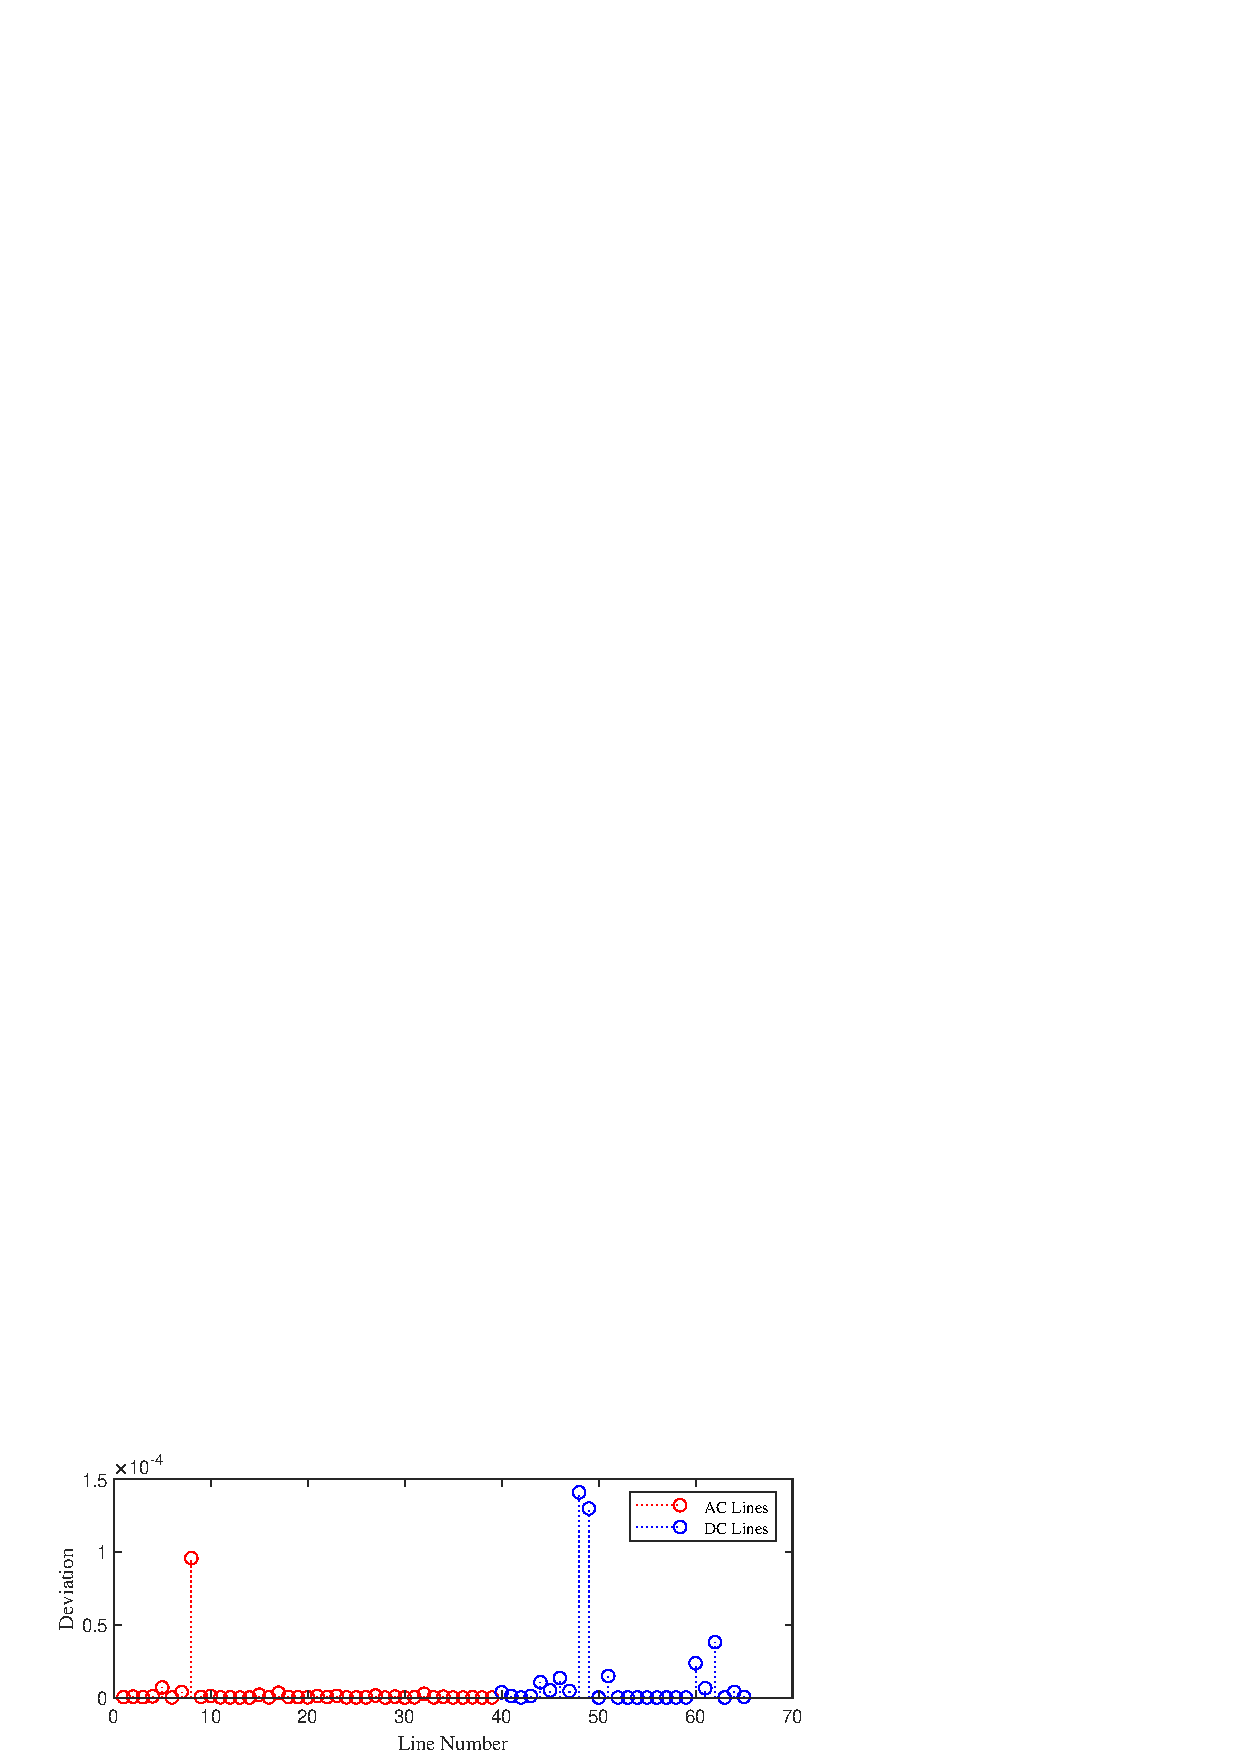
\includegraphics[width = 3.3 in]{image_files/error.png}
    \caption{\textrm{{\color{blue}
    Deviations of Second Order Conic Relaxations for AC and DC systems.}}}
    \label{error}
\end{figure}

In the proposed planning strategy, a novel contingency screening approach is 
developed to check the N-1 security criterion. Since the efficiency of 
contingency screening has a significant influence on the solving speed of the 
planning model, the superiority of the proposed screening strategy is 
further illustrated. Here, the method in \cite{Lin_2019_Distribution} is 
adopted as the benchmark for comparison, where the CPU run-time for the 
contingency screening in each iteration is logged. The result is listed in 
Table \ref{tab_algorithm}.

As can be seen, the proposed algorithm outperforms the benchmark with an 
efficiency improvement more than 50\%. The main reason is that the benchmark 
method in \cite{Lin_2019_Distribution} has to check every N-1 contingency 
in the contingency set, while the screening approach in this paper is 
conducted based on an iterative optimization, which avoids massive unnecessary 
calculation.
}

{\color{blue}
\subsection{Effectiveness of Conic Relaxation}

To verify the effectiveness of the SOCP-based AC-DC OPF model, the deviations 
of the conic relaxation constraints (\ref{s_bfm_AC}) and (\ref{s_bfm_DC}) are 
denoted by $ \epsilon_{m} $ calculated by
\begin{align}
    \epsilon_{m} =
    \left\{\!\!
        \begin{array}{lr}
        \sum\limits_{c,h,t} \left| l_{m,c,h,t} - 
        \frac{(p_{m,c,h,t}^{l})^{2} + (q_{m,c,h,t}^{l})^{2}}
        {v_{se(m),c,h,t}} \right| \!, 
        & \!\!\!\! {\rm if} \ m \in \Omega_{l}^{AC} \\
        \sum\limits_{c,h,t} \left| l_{m,c,h,t} - 
        \frac{(p_{m,c,h,t}^{l})^{2}}{v_{se(m),c,h,t}} \right| \!, 
        & \!\!\!\! {\rm if} \ m \in \Omega_{l}^{DC}
        \end{array}
    \right.
\end{align}

\noindent where the absolute error of the conic relaxation is adopted to 
quantified the validity of the model. The distribution of $ \epsilon_{m} $
is shown in Fig. \ref{error}. As can be seen, the errors are in the order of
$ 10^{-4} $, which indicates that the relaxations in (\ref{s_bfm_AC}) and 
(\ref{s_bfm_DC}) are tight.

}

\section{Conclusion}

This paper proposes a security-constrained AC/DC hybrid distribution system 
planning model for accommodating high penetration of renewable energy in weak 
distribution systems. The network reconfiguration under both normal and 
contingency states are jointly considered. To alleviate the computational 
burden, a nested loop-based solving structure is developed to iteratively 
filter the security constraints based on a novel contingency screening 
approach.

The proposed planning model and solving methodology are tested on a 
real-world distribution network in Zhejiang Province, China. The planning 
results indicate that the AC-DC hybrid distribution system is a promising 
approach for the accommodation of large-scale renewable energy in weak 
distribution systems. Numerical results further illustrate the effectiveness 
and superiority of the proposed 
{\color{blue}
model and the novel contingency screening strategy.

Further research will focus on the improvements of the contingency screening 
approach based on the lazy constraint callback technology.
}

\section*{Acknowledgement}

This work is supported by the Funds for International Cooperation and Exchange 
of the National Natural Science Foundation of China (Grant No. 52061635104).

\bibliographystyle{cas-num-names}
\bibliography{reference}

{\color{blue}
\section*{Appendices}

\subsection*{A. Lower and Upper Bounds}

\setcounter{equation}{0}
\renewcommand{\theequation}{A.\arabic{equation}}

The lower and upper boundaries of variables are given as follows.
\begin{align}
    \label{v_bound}
    - \bigl( V_{n}^{\min} \bigr)^{2} 
    \leq v_{n,c,h,t} 
    \leq \bigl( V_{n}^{\max} \bigr)^{2},
    \quad \forall n \in \Omega_{b}, \forall c,h,t
\end{align}
\begin{align}
    \label{i_bound}
    0
    \leq l_{m,c,h,t} 
    \leq \bigl( L_{m}^{\max} \bigr)^{2} y_{br(m),c,h,t}^{r},
    \quad \forall m \in \Omega_{l}, \forall c,h,t
\end{align}
\begin{align}
    \label{p_line_onoff}
    \left| p_{m,c,h,t}^{l} \right| \leq S_{m}^{l, \max} y_{br(m),c,h,t}^{r},
    \ \, \forall m \in \Omega_{l}, 
    \forall c,h,t
\end{align}
\begin{align}
    \label{q_line_onoff}
    \left| q_{m,c,h,t}^{l} \right| \leq S_{m}^{l, \max} y_{br(m),c,h,t}^{r},
    \ \, \forall m \in \Omega_{l}, 
    \forall c,h,t
\end{align}
\begin{align}
    \label{p_line_ext}
    -S_{m}^{l, \max} \leq p_{m,c,h,t}^{l} \leq S_{m}^{l, \max},
    \quad \forall m \in \Omega_{l}^{e}, \forall c,h,t
\end{align}
\begin{align}
    \label{q_line_ext}
    -S_{m}^{l, \max} \leq q_{m,c,h,t}^{l} \leq S_{m}^{l, \max},
    \quad \forall m \in \Omega_{l}^{e}, \forall c,h,t
\end{align}
\begin{align}
    \label{p_line_cdd}
    -S_{m}^{l, \max} x_{m,t}^{l} \leq p_{m,c,h,t}^{l} \leq S_{m}^{l, \max} x_{m,t}^{l},
    \forall m \in \Omega_{l}^{c}, \forall c,h,t
\end{align}
\begin{align}
    \label{q_line_cdd}
    -S_{m}^{l, \max} x_{m,t}^{l} \leq q_{m,c,h,t}^{l} \leq S_{m}^{l, \max} x_{m,t}^{l},
    \forall m \in \Omega_{l}^{c}, \forall c,h,t
\end{align}
\begin{align}
    \label{p_VSC_ext}
    S_{m}^{v, \min} \leq p_{m,c,h,t}^{v} \leq S_{m}^{v, \max},
    \quad \forall m \in \Omega_{v}^{e}, \forall c,h,t
\end{align}
\begin{align}
    \label{q_VSC_ext}
    S_{m}^{v, \min} \leq q_{m,c,h,t}^{v} \leq S_{m}^{v, \max},
    \quad \forall m \in \Omega_{v}^{e}, \forall c,h,t
\end{align}
\begin{align}
    \label{p_VSC_cdd}
    S_{m}^{v, \min} x_{m,t}^{v} \leq p_{m,c,h,t}^{v} \leq S_{m}^{v, \max} x_{m,t}^{v},
    \forall m \in \Omega_{v}^{c}, \forall c,h,t
\end{align}
\begin{align}
    \label{q_VSC_cdd}
    S_{m}^{v, \min} x_{m,t}^{v} \leq q_{m,c,h,t}^{v} \leq S_{m}^{v, \max} x_{m,t}^{v},
    \forall m \in \Omega_{v}^{c}, \forall c,h,t
\end{align}
\begin{align}
    \label{p_DG_ext}
    0 \leq p_{n,c,h,t}^{g} \leq S_{n}^{g, \max} \varphi_{n,h,t}^{p},
    \quad \forall n \in \Omega_{g}^{e}, \forall c,h,t
\end{align}
\begin{align}
    \label{q_DG_ext}
    \left| q_{n,c,h,t}^{g} \right| \leq 
    S_{n}^{g, \max} \varphi_{n,h,t}^{q},
    \quad \forall n \in \Omega_{g}^{e}, \forall c,h,t
\end{align}
\begin{align}
    \label{p_DG_cdd}
    0 \leq p_{n,c,h,t}^{g} \leq S_{n}^{g, \max} \varphi_{n,h,t}^{p} x_{n,t}^{g},
    \quad \forall n \in \Omega_{g}^{c}, \forall c,h,t
\end{align}
\begin{align}
    \label{q_DG_cdd}
    \left| q_{n,c,h,t}^{g} \right| \leq 
    S_{n}^{g, \max} \varphi_{n,h,t}^{q} x_{n,t}^{g},
    \quad \forall n \in \Omega_{g}^{c}, \forall c,h,t
\end{align}
\begin{align}
    \label{p_sub_ext}
    0 \leq p_{n,c,h,t}^{s} \leq S_{n}^{s, \max},
    \quad \forall n \in \Omega_{s}^{e}, \forall c,h,t
\end{align}
\begin{align}
    \label{q_sub_ext}
    0 \leq q_{n,c,h,t}^{s} \leq S_{n}^{s, \max},
    \quad \forall n \in \Omega_{s}^{e}, \forall c,h,t
\end{align}
\begin{align}
    \label{p_sub_cdd}
    0 \leq p_{n,c,h,t}^{s} \leq S_{n}^{s, \max} x_{n,t}^{s},
    \quad \forall n \in \Omega_{s}^{c}, \forall c,h,t
\end{align}
\begin{align}
    \label{q_sub_cdd}
    0 \leq q_{n,c,h,t}^{s} \leq S_{n}^{s, \max} x_{n,t}^{s},
    \quad \forall n \in \Omega_{s}^{c}, \forall c,h,t
\end{align}
\begin{align}
    \label{p_shed}
    0 \leq p_{n,c,h,t}^{u} \leq D_{n,h,t}^{p},
    \quad \forall n \in \{\Omega_{b}^{AC} \cup \Omega_{b}^{DC}\},
    \forall c,h,t
\end{align}
\begin{align}
    \label{q_shed}
    0 \leq q_{n,c,h,t}^{u} \leq D_{n,h,t}^{q},
    \quad \forall n \in \Omega_{b}^{AC},
    \forall c,h,t
\end{align}

Constraint (\ref{v_bound}) refers to 
the lower and upper bounds of bus voltage and constraint (\ref{i_bound})
sets the lower and upper bounds of line current. Constraints 
(\ref{p_line_onoff})-(\ref{q_line_onoff}) mean that the power flow on the 
switch-off branch is forced to $ 0 $. Constraints
(\ref{p_line_ext})-({\ref{q_line_cdd}}) represent the lower and upper limits
of power flow on the existing and candidate lines, 
(\ref{p_VSC_ext})-({\ref{q_VSC_cdd}}) are the power conversion limits of
VSCs. The active and reactive power generation of renewable DGs are restricted
in (\ref{p_DG_ext})-({\ref{q_DG_cdd}}) based on the forecasted values. In
(\ref{p_sub_ext})-(\ref{q_sub_cdd}), the power injection from substation is 
restricted to the rated capacity. The ranges of load 
shedding are given in (\ref{p_shed}) and (\ref{q_shed}).
}

{\color{blue}
\subsection*{B. Key System Parameters}

The parameters of the real-world distribution system are given in Table 
\ref{tab_load} to Table \ref{tab_cost_dgs}.

}

\setcounter{table}{0}
\renewcommand{\thetable}{B.\arabic{table}}

% data of load
\begin{table*}[htbp]\footnotesize
    \renewcommand{\familydefault}{\rmdefault}\normalfont
    \renewcommand{\arraystretch}{1.1}
    \setlength\tabcolsep{5pt}
    \centering
    {\color{blue}
    \caption{\textrm{Data of Nodal Load (MVA)}}
    \begin{tabularx}{\linewidth}{c|YYY|c|YYY|c|YYY|c|YYY}
    \hline
    \multirow{2}[0]{*}{No.} & \multicolumn{3}{c|}{Stage} & 
    \multirow{2}[0]{*}{No.} & \multicolumn{3}{c|}{Stage} & 
    \multirow{2}[0]{*}{No.} & \multicolumn{3}{c|}{Stage} & 
    \multirow{2}[0]{*}{No.} & \multicolumn{3}{c}{Stage} \\
    \cline{2-4}
    \cline{6-8}
    \cline{10-12}
    \cline{14-16}
        & 1      & 2      & 3      &       & 1      & 2      & 3 & 
        & 1      & 2      & 3      &       & 1      & 2      & 3 \\
    \hline
    1   & 0      & 0      & 0      & 16    & 18.70  & 23.86  & 30.45  & 
    31  & 17.51  & 22.34  & 28.51  & 46    & 0      & 17.89  & 27.65  \\
    2   & 0      & 0      & 0      & 17    & 47.70  & 60.87  & 77.66  & 
    32  & 6.86   & 8.75   & 11.17  & 47    & 0      & 0      & 25.08  \\
    3   & 0      & 0      & 0      & 18    & 0      & 0      & 0     & 
    33  & 21.88  & 27.92  & 35.62  & 48    & 14.61  & 19.72  & 26.63  \\
    4   & 64.98  & 82.91  & 105.80 & 19    & 0      & 0      & 0     & 
    34  & 0      & 0      & 0      & 49    & 20.20  & 27.27  & 36.81  \\
    5   & 20.50  & 26.16  & 33.38  & 20    & 0      & 0      & 0     & 
    35  & 0      & 0      & 0      & 50    & 0      & 14.64  & 19.76  \\
    6   & 42.70  & 54.49  & 69.52  & 21    & 20.58  & 26.26  & 33.51  & 
    36  & 0      & 0      & 0      & 51    & 14.20  & 19.17  & 25.88  \\
    7   & 13.60  & 17.35  & 22.14  & 22    & 18.75  & 23.93  & 30.53  & 
    37  & 0      & 0      & 0      & 52    & 0      & 0      & 17.39  \\
    8   & 57.96  & 73.96  & 94.37  & 23    & 7.62   & 9.72   & 12.41  & 
    38  & 0      & 0      & 0      & 53    & 0      & 0      & 0 \\
    9   & 36.10  & 46.06  & 58.78  & 24    & 2.93   & 3.74   & 4.77  & 
    39  & 0      & 0      & 0      & 54    & 4.69   & 6.33   & 8.55  \\
    10  & 28.50  & 36.37  & 46.40  & 25    & 7.95   & 10.14  & 12.94  & 
    40  & 0      & 0      & 0      & 55    & 0      & 4.73   & 6.38  \\
    11  & 73.60  & 93.91  & 119.83 & 26    & 0      & 0      & 0     & 
    41  & 0      & 0      & 0      & 56    & 0      & 0      & 3.50  \\
    12  & 101.01 & 128.89 & 164.46 & 27    & 3.40   & 4.34   & 5.54  & 
    42  & 0      & 0      & 0      & 57    & 0      & 4.38   & 5.91  \\
    13  & 32.60  & 41.60  & 53.08  & 28    & 0      & 0      & 0     & 
    43  & 0      & 0      & 0      &       &        &        &   \\
    14  & 73.20  & 93.40  & 119.18 & 29    & 19.23  & 24.54  & 31.31  & 
    44  & 0      & 0      & 0      &       &        &        &   \\
    15  & 71.00  & 90.60  & 115.60 & 30    & 23.45  & 29.92  & 38.18  & 
    45  & 0      & 0      & 0      &       &        &        &   \\
    \hline    
    \end{tabularx}
    \label{tab_load}
    }
\end{table*}

% data of AC/DC lines
\begin{table}[htbp]\footnotesize
    \renewcommand{\familydefault}{\rmdefault}\normalfont
    \renewcommand{\arraystretch}{1.1}
    \setlength\tabcolsep{1pt}
    \centering
    {\color{blue}
    \caption{\textrm{Data of AC and DC Lines}}
    \begin{tabularx}{\columnwidth}{YYYcY|YYYcY}
    \hline
    No.   & From  & To    & Length (km)   & Type  & 
    No.   & From  & To    & Length (km)   & Type \\
    \hline
    1     & 1     & 9     & 11.1  & AC    & 40    & 28    & 29    & 7.84  & AC \\
    2     & 1     & 10    & 5.1   & AC    & 41    & 31    & 32    & 8.44  & AC \\
    3     & 1     & 12    & 7.1   & AC    & 42    & 32    & 33    & 4.59  & AC \\
    4     & 1     & 13    & 5.82  & AC    & 43    & 33    & 45    & 9.47  & AC \\
    5     & 1     & 14    & 3.24  & AC    & 44    & 34    & 35    & 5.9   & DC \\
    6     & 1     & 15    & 6.3   & AC    & 45    & 34    & 47    & 10.42 & DC \\
    7     & 1     & 18    & 21.32 & AC    & 46    & 34    & 49    & 19.37 & DC \\
    8     & 1     & 19    & 29.56 & AC    & 47    & 35    & 37    & 6.18  & DC \\
    9     & 1     & 26    & 10.93 & AC    & 48    & 36    & 37    & 9.32  & DC \\
    10    & 1     & 27    & 10.42 & AC    & 49    & 36    & 41    & 18.5  & DC \\
    11    & 1     & 28    & 27.44 & AC    & 50    & 36    & 53    & 27.26 & DC \\
    12    & 1     & 29    & 21.92 & AC    & 51    & 37    & 55    & 19.25 & DC \\
    13    & 1     & 30    & 24.43 & AC    & 52    & 38    & 39    & 5.58  & DC \\
    14    & 2     & 4     & 8.88  & AC    & 53    & 38    & 40    & 4.57  & DC \\
    15    & 2     & 5     & 4.77  & AC    & 54    & 38    & 55    & 27.28 & DC \\
    16    & 2     & 6     & 11.58 & AC    & 55    & 39    & 40    & 3.82  & DC \\
    17    & 2     & 8     & 10.92 & AC    & 56    & 39    & 42    & 4.27  & DC \\
    18    & 2     & 9     & 8.73  & AC    & 57    & 39    & 44    & 5.98  & DC \\
    19    & 2     & 10    & 12.76 & AC    & 58    & 39    & 56    & 10.31 & DC \\
    20    & 2     & 21    & 11.12 & AC    & 59    & 40    & 41    & 3.56  & DC \\
    21    & 3     & 8     & 23.62 & AC    & 60    & 40    & 42    & 4.22  & DC \\
    22    & 3     & 16    & 4.52  & AC    & 61    & 41    & 43    & 4.95  & DC \\
    23    & 3     & 17    & 4.97  & AC    & 62    & 42    & 43    & 3.41  & DC \\
    24    & 3     & 20    & 15.14 & AC    & 63    & 42    & 44    & 4.22  & DC \\
    25    & 3     & 31    & 12.29 & AC    & 64    & 44    & 57    & 10.3  & DC \\
    26    & 4     & 5     & 4.5   & AC    & 65    & 46    & 49    & 7.1   & DC \\
    27    & 4     & 21    & 15.39 & AC    & 66    & 46    & 50    & 3.24  & DC \\
    28    & 6     & 22    & 3.5   & AC    & 67    & 46    & 51    & 6.3   & DC \\
    29    & 7     & 8     & 7.17  & AC    & 68    & 47    & 52    & 4.97  & DC \\
    30    & 9     & 11    & 4.18  & AC    & 69    & 47    & 55    & 12.29 & DC \\
    31    & 9     & 24    & 7.89  & AC    & 70    & 48    & 49    & 3.87  & DC \\
    32    & 11    & 12    & 3.87  & AC    & 71    & 48    & 52    & 20.84 & DC \\
    33    & 11    & 23    & 3.51  & AC    & 72    & 49    & 51    & 5.7   & DC \\
    34    & 13    & 14    & 4.82  & AC    & 73    & 50    & 51    & 4.09  & DC \\
    35    & 15    & 17    & 24.22 & AC    & 74    & 51    & 54    & 19.21 & DC \\
    36    & 17    & 33    & 18.69 & AC    & 75    & 52    & 57    & 18.69 & DC \\
    37    & 19    & 30    & 6.26  & AC    & 76    & 53    & 54    & 6.26  & DC \\
    38    & 23    & 24    & 2.88  & AC    & 77    & 55    & 56    & 8.44  & DC \\
    39    & 25    & 26    & 12.55 & AC    & 78    & 56    & 57    & 4.59  & DC \\
    \hline
    \end{tabularx}
    \label{tab_line}
    }
\end{table}
  
% data of VSC stations
\begin{table}[htbp]\footnotesize
    \renewcommand{\familydefault}{\rmdefault}\normalfont
    \renewcommand{\arraystretch}{1.1}
    \setlength\tabcolsep{3pt}
    \centering
    {\color{blue}
    \caption{\textrm{Data of VSC Stations}}
    \begin{tabularx}{\columnwidth}{YYYcYYYc}
    \hline
    VSC   & From  & To    & Capacity   & VSC  & From    & To   & Capacity \\
    \hline
    1     & 1     & 46    & 100 MVA & 7     & 17    & 52   & 100 MVA \\
    2     & 3     & 47    & 100 MVA & 8     & 19    & 53   & 100 MVA \\
    3     & 11    & 48    & 100 MVA & 9     & 30    & 54   & 100 MVA \\
    4     & 12    & 49    & 100 MVA & 10    & 31    & 55   & 100 MVA \\
    5     & 14    & 50    & 100 MVA & 11    & 32    & 56   & 100 MVA \\
    6     & 15    & 51    & 100 MVA & 12    & 33    & 57   & 100 MVA \\  
    
    \hline
    \end{tabularx}
    \label{tab_VSC}
    }
\end{table}

% data of renewable DGs
\begin{table}[htbp]\footnotesize
    \renewcommand{\familydefault}{\rmdefault}\normalfont
    \renewcommand{\arraystretch}{1.1}
    \setlength\tabcolsep{5pt}
    \centering
    {\color{blue}
    \caption{\textrm{Data of Renewable DGs}}
    \begin{tabularx}{\columnwidth}{YYccYYcc}
    \hline
    DG    & Bus   & Capacity  & Type  & DG & Bus & Capacity & Type \\
    \hline
    1     & 18    & 48 MW     & Wind  & 10 & 38  & 30 MW     & Solar \\
    2     & 19    & 99 MW     & Solar & 11 & 39  & 30 MW     & Solar \\
    3     & 20    & 58.5 MW   & Wind  & 12 & 40  & 45 MW     & Solar \\
    4     & 26    & 5 MW      & Hydro & 13 & 41  & 25 MW     & Wind \\
    5     & 28    & 18 MW     & Hydro & 14 & 42  & 45 MW     & Solar \\
    6     & 34    & 20 MW     & Solar & 15 & 43  & 25 MW     & Wind \\
    7     & 35    & 20 MW     & Solar & 16 & 44  & 30 MW     & Solar \\
    8     & 36    & 80 MW     & Solar & 17 & 45  & 55 MW     & Hydro \\
    9     & 37    & 35 MW     & Wind  &    &     &           &  \\
    \hline
    \end{tabularx}
    \label{tab_gen}
    }
\end{table}

% data of substations
\begin{table}[htbp]\footnotesize
    \renewcommand{\familydefault}{\rmdefault}\normalfont
    \renewcommand{\arraystretch}{1.1}
    \setlength\tabcolsep{5pt}
    \centering
    {\color{blue}
    \caption{\textrm{Data of Substations}}
    \begin{tabularx}{\columnwidth}{ccYYc}
    \hline
    Substation & Bus   & Capacity & Expansion & Transformation Ratio \\
    \hline
    1     & 1     & 360 MVA   & 120 MVA   & 220/110/35 \\
    2     & 2     & 360 MVA   & 120 MVA   & 220/110/35 \\
    3     & 3     & 480 MVA   & 120 MVA   & 220/110/35 \\
    \hline
    \end{tabularx}
    \label{tab_sub}
    }
\end{table}

% parameter of lines
\begin{table}[!t]\footnotesize
    \renewcommand{\familydefault}{\rmdefault}\normalfont
    \renewcommand{\arraystretch}{1.1}
    \setlength\tabcolsep{4pt}
    \centering
    {\color{blue}
    \caption{\textrm{Parameters of Candidate AC/DC Lines}}
    \begin{tabularx}{\columnwidth}{cccYYc}
    \hline
    Type  & Model   & Capacity & Resistance & Reactance & Cost \\
    \hline
    AC    & LGJ-240 & 120 MVA  & 0.36 $\Omega$/km & 0.13 $\Omega$/km & $ \yen $ 8.7$\times 10^5$/km \\
    DC    & LGJ-185 & 90 MVA   & 0.36 $\Omega$/km & 0.00 $\Omega$/km & $ \yen $ 4.7$\times 10^5$/km \\
    AC    & LGJ-150 & 30 MVA   & 0.37 $\Omega$/km & 0.21 $\Omega$/km & $ \yen $ 2.6$\times 10^5$/km \\
    \hline
    \end{tabularx}
    \label{tab_cost_line}
    }
\end{table}

% parameter of VSCs
\begin{table}[!t]\footnotesize
    \renewcommand{\familydefault}{\rmdefault}\normalfont
    \renewcommand{\arraystretch}{1.1}
    \setlength\tabcolsep{2pt}
    \centering
    {\color{blue}
    \caption{\textrm{Parameters of Candidate VSC Stations}}
    \begin{tabularx}{\columnwidth}{cYYYc}
    \hline
    Model      & AC Voltage & DC Voltage & Capacity & Cost \\
    \hline
    HVDC-light & 110 kV & $ \pm $50 kV & 100 MVA  & $ \yen $ 1.0278 $\times 10^8$ \\
    \hline
    \end{tabularx}
    \label{tab_cost_VSC}
    }
\end{table}

% parameter of substations
\begin{table}[htbp]\footnotesize
    \renewcommand{\familydefault}{\rmdefault}\normalfont
    \renewcommand{\arraystretch}{1.1}
    \setlength\tabcolsep{8pt}
    \centering
    {\color{blue}
    \caption{\textrm{Parameters of Candidate Substations}}
    \begin{tabularx}{\columnwidth}{cccc}
    \hline
    Type  & Model & Capacity & Cost of Expansion \\
    \hline
    1    & OSFPSZ-180000/220 & 180 MVA  & $ \yen $ 2.41 $\times 10^7$ \\
    2    & OSFPSZ-150000/220 & 150 MVA  & $ \yen $ 2.01 $\times 10^7$ \\
    3    & OSFPSZ-120000/220 & 120 MVA  & $ \yen $ 1.61 $\times 10^7$ \\
    \hline
    \end{tabularx}
    \label{tab_cost_subs}
    }
\end{table}

% parameter of DGs
\begin{table}[htbp]\footnotesize
    \renewcommand{\familydefault}{\rmdefault}\normalfont
    \renewcommand{\arraystretch}{1.1}
    \setlength\tabcolsep{5pt}
    \centering
    {\color{blue}
    \caption{\textrm{Parameters of Candidate Renewable DGs}}
    \begin{tabularx}{\columnwidth}{cccc}
    \hline
    Type   & Model & Investment Cost & Operating Cost \\
    \hline
    Wind   & WD103-2000T       & $ \yen $ 8.032 $\times 10^6$/MW & $ \yen $ 22/MWh \\
    Solar  & RSM72-6-325P-345P & $ \yen $ 7.099 $\times 10^6$/MW & $ \yen $ 17/MWh \\
    Hydro  & GZF02-WP          & $ \yen $ 6.643 $\times 10^6$/MW & $ \yen $ 67/MWh \\
    \hline
    \end{tabularx}
    \label{tab_cost_dgs}
    }
\end{table}

\end{document}